
\chapter{Human-Robot Handovers using Task-Space Quadratic Programming}\label{chap:handover qp}

%\begin{itemize}
%	\item Figure of task interdependency 
%\end{itemize}

In the previous chapter, we addressed the issue of constraints compatibility between the hardware limitations and kinematic constraints. Since this issue requires a look-ahead on the robot motion, our idea consisted of enhancing the reactive whole-body QP by an MPC-based reference governor. We showed how the latter modifies the tasks' references to ensure compatibility between constraints.

%In the previous chapter, we proposed a robust feedback closed-loop QP control formulation in the case of kinematic-controlled robots. Task and set robust stability have been formally proved and validated in real experiments. In the case of multi-objective control, robust stability of relaxed tasks has been also proved. 

Multi-objective control is the main beneficial property exploited from the robot's redundancy. This control paradigm enabled the robots to execute more than one task, thereby approaching the natural human abilities. More importantly,  it opened wide the field for robots to get involved in plenty of domains, which has increased their impact on the economy, education, health service quality, food delivery, ergonomy, tourism, etc. In particular, one of the currently very active trends in robotics is maximizing the interactions between humans and robots. Among the most challenging ones, seamlessly exchanging objects between a human and robot as \emph{giver} and \emph{receiver} agents through (bi-directional) handovers is of the most importance (\cref{fig:handover examples}). Indeed, handing objects between humans is a persistent daily interaction in almost all domains~\cite{ortenzi2021tro}. Therefore, embedding human-centered robotic systems in automation and services with handovers capabilities is a key enabler for rich cognitive interaction~\cite{ajoudani2018autonomousRobots,billard2019science}. Although human-human handover is an intuitive behavior, it is a result of complex and sophisticated learned social-cognitive communication channels~\cite{strabala2013jhrisc}. Grasping such complexity in an equivalent robot control formulation strategy is not a trivial problem.

In this chapter, we formulate the premises of a generic robot control-strategy that ensures high fidelity and reliability of reaching motion for bi-directional handover scenarios and guarantees adaptability w.r.t the handover location (HOL, i.e., the meeting point where the two handover agents exchange the object) as well as the object orientation. Particularly, our control formulation is handover-location knowledge free. We only assume that the object's structural properties and dimensions are known, and there exists a sensor that tracks the pose (Cartesian position and orientation) of the object in interest, e.g.~\cite{paolillo2018ral}. In \cref{sec-chap4:sota}, we go through the state-of-the-art of human-robot handover control formulations and their limitations which enables us to present our contribution in \cref{subsec-chap4:contribution} succinctly. Then, we present in \cref{sec-chap4:handover formulation} the details of our task-space QP-based handover controller. Finally, we implement our method on Panda robotic arm taking objects from a human operator in \cref{sec-chap4:experiments}. 
%\textbf{Keep this as a result}The proposed control formulation ensures a real-time adaptation of the robot to the human desired HOL and orientation. 
%Of course, our first constraints is to build on our existing task-space optimization (QP) formulation framework~\cite{bouyarmane2018tac,bouyarmane2019tro} that prove to be very powerful in an industrial context~\cite{kheddar2019ram} and a human-assistance context~\cite{bolotnikova2021sii}. 



%Remove some references...

\section{Human-Robot Handover: State-of-The-Art}\label{sec-chap4:sota}
How to \emph{codify} the human-robot handover process has been thoroughly addressed in the research community. The state of the art studies split the handover process in two main phases: the \emph{pre-grasping} phase~\cite{shibata1995roman,waldhart2015iros,mainprice2021roman,huber2008roman,shi2013rss,koene2014roman,remazeilles2015rss} and the \emph{grasping} phase~\cite{nagata1998icra,chan2013ijrr,medina2016humanoids,solak2019iros,costanzo2021frontiersRob-AI}.
%\begin{itemize}
%	\item  \emph{Pre-grasping phase}~\cite{shibata1995roman,waldhart2015iros,mainprice2021roman,huber2008roman,shi2013rss,koene2014roman,remazeilles2015rss}
%	\item \emph{Grasping phase}~\cite{nagata1998icra,chan2013ijrr,medina2016humanoids,solak2019iros,costanzo2021frontiersRob-AI}
%\end{itemize} 
Such a breakdown is chronological: the former focuses on estimating/predicting the human movement and planning the robot reaching motion toward the meeting point, whereas the latter consists of understanding the interaction forces (haptics) applied at the object by the two handing over agents during the exchange such that to ensure a stable grasping. In~\cite{medina2016humanoids} a \emph{retraction} phase is considered, which describes how the giver and receiver move away after the latter gets full control of the object. In this chapter, we are interested in the pre-grasping phase of the handover process. Yet, for an exhaustive handover survey, please refer to the excellent recent review in~\cite{ortenzi2021tro}.  

\begin{figure}
	\centering
	\includegraphics[width=0.65\columnwidth]{collage3}
	\caption{Different handover scenarios: handing food for patient (top-left~\cite{nemlekar2019icra}), sharing a tool for a mechanic (top-right~\cite{prada2014iros}), lending mustard (bottom-left~\cite{ortenzi2021tro}), giving a water bottle (bottom-right~\cite{medina2016humanoids}).}
	\label{fig:handover examples}
\end{figure}

The pre-grasping phase formulation involves two subsequent questions: (i) \emph{where} and \emph{when} the handover will take place; (ii) how to generate the reaching motion.  \emph{Where} to handover is denoted as the HOL (also known as the object transfer point~\cite{li2015rss,nemlekar2019icra}), whereas \emph{when} to handover depends on the agents synchronization to reach the handover location, and the elapsed time during the object release by the giver and the full object control by the receiver. Planning for the reaching phase (ii) depends highly on the HOL knowledge. 

Different approaches have been proposed to formulate the robot's reaching motion. Dynamic Movement Primitives (DMP) are among the most documented and well theoretically-grounded methods. They were introduced in~\cite{ijspeert2002icra,schaal2005springer} as a powerful tool to generate complex trajectories while converging to a goal-attractor. DMP have been recently exploited to learn from demonstration and generate human-like handover robotic movement~\cite{prada2014iros}, and to predict the HOL and time using an extended Kalman Filter~\cite{widmann2018ecc}. The drawback of DMP-based approaches is the high number of hyper-parameter to tune, especially in high dimensions. In addition, the use of DMP as a part of a closed-loop system has been barely studied where the majority of works consider it a planning block only forwarding the references for the controller~\cite{saveriano2021arxiv}.
Probabilistic Movement Primitives (Pro-MP), which is an extension of DMP to stochastic systems~\cite{paraschos2013anips}, have been used in~\cite{nemlekar2019icra} to estimate the HOL dynamically from the observed human motion. However, the resulting motion is not fluent, and the robot does not well anticipate the object. 

\cite{laplaza2021roman} used video recordings of robot-human handover to train an attention deep-learning model that predicts the human joint positions. However, no further details have been provided about how this prediction is used for the robot reaching-motion formulation. Based on vision object-recognition, using eye-in-hand vision,~\cite{rosenberger2021ral} proposed an object-independent approach that does not require the prior knowledge of the object dimension/shape. A gripper-mounted camera is used to detect and distinguish between the human agent's hand and the object leveraging a trained image-classifier. It also enables a safe grasping and gripper orientation. However, the approach is computationally demanding and suffers a high time response to detect the object, which is constrained to remain static. Eye-in-hand vision has also been adopted in~\cite{costanzo2021frontiersRob-AI} except that the approach is based on reactive visual servoing. The latter generates robot motion to minimize the error between the perceived object image and a priorly acquired image.
Interestingly, the HOL knowledge is not required for the control formulation. However, an image database of the exchanged objects must be collected priorly. In addition, the experiment showed that the robot motion is not sufficiently proactive because of the low image-sampling frequency, and the object must be inside the camera field-of-view. 

\cite{medina2016humanoids} trained a Dynamical System (DS) to predict the human motion based on real-time motion data observed during a time window. The HOL is estimated online to be the robot's closest point (among the predicted human trajectory). 
The handover controller is formulated as two coupled dynamical systems: the giver (master) converges to the estimated HOL, and the receiver converges to an attractor that depends on the master convergence error.
%Then, the closest point to the robot among the predicted trajectory is considered as the handover location. Two Dynamical systems for the human hand and robot end-effector motion modeling are learned from offline experiment data. Then, handover controller is formulated as a coupled dynamical systems: the giver (master) converges to the estimated handover location, and the receiver converges to an attractor that depends on the master convergence error. Two dynamical systems are also learned for the angular motion modeling for both human hand and robot end-effectors. Which is time consuming for collecting data.

%Discuss how the motion during the pre-grasping phase is generated: DMP, Planning, DS, etc. 


%Despite the huge amount of works addressing human-robot handover, one issue remains open: how to ensure/codify an adaptive behavior of the robot w.r.t to a human versatile intention on \emph{where} to exchange the object, aka \emph{HandOver Location} (HOL), with the robot, and in which configuration (\emph{orientation}).  
Many existing works required the knowledge of the HOL as a precondition for motion planning or control formulations of the pre-grasping phase. In particular, the HOL is often considered either as fixed (the robot moves systematically to a fixed spot to pick up the object) or pre-planned (real-time detection and estimation of the object's fixed location) (see Tables~1~\&~2 in~\cite{ortenzi2021tro}). There are works that provide HOL estimation and online prediction methods~\cite{prada2014iros,medina2016humanoids,vahrenkamp2016humanoids,maeda2017autonomousRobots,widmann2018ecc,nemlekar2019icra}. However, such existing approaches have at least one of the following shortcomings:
\begin{itemize}
	\item Collecting data sets to train motion prediction models;
	\item Time-consuming computations leading to a hashed or a slow handover motion; 
	\item Magic-numbers of hyper-parameters to tune;
	\item Conservatism in the handover-location prediction policy; 
	\item Non-systematic success of the handover performance (i.e., success rates);
	\item The object orientation at the HOL is often kept the same during the experiments;
	\item Knowledge of the HOL is required.
\end{itemize}
\subsection{Contribution}\label{subsec-chap4:contribution}
Our proposed approach is meant to mitigate the above issues. More concretely, it gathers the advantages from both methods in~\cite{costanzo2021frontiersRob-AI,medina2016humanoids}. Indeed, our handover formulation does not require the knowledge of the HOL. Conversely to~\cite{costanzo2021frontiersRob-AI}, our method ensures/codifies a real-time proactive and adaptive robot motion w.r.t the human versatile intention on \emph{where} to exchange the object with the robot and in which configuration (\emph{orientation}). In fact, our proposed idea relies on the concept of \emph{interdependent tasks} where the state of one task is forwarded as the reference for another task. More precisely, we formulate an \emph{observation task} that estimates either the human hand or object full-state (depending on who is the giver) in terms of pose, velocity and acceleration which are then forwarded as references for a \emph{trajectory-tracking task} for the robot end-effector to track. Leveraging multi-objective QP control paradigm, these two tasks run concurrently in a leader-follower fashion: the object (leader) moves and converges to the HOL while the robot end-effector (follower) moves proactively toward the object while adjusting its orientation accordingly. From this standpoint, our approach is similar to the coupled DS in~\cite{medina2016humanoids}. Conversely, our approach is computationally cheap and does not require the estimation of the HOL or separately learning human and robot DS models.
\section{Task-Space QP Handover Formulation}\label{sec-chap4:handover formulation}
In this section, we first explain our methodology. Then, we detail our handover control formulation.
\subsection{Handover Control Problem}
%In order to achieve object handover efficiently, the robot reaching-motion toward the HOL shall be synchronized with the object's motion to have a \emph{one-shot continuous and smooth motion}. If the HOL is known in advance, the control formulation resumes to perform simply a set-point task for the end-effector (eventually with a secondary pre-planned trajectory tracking task). Nevertheless, the HOL as well as the object orientation are highly versatile: they may change during the handover motion or between two successive processes depending on the human intention and her/his posture. Handing over an object can even be aborted by a human decision while moving. Hence, planning the robot motion is likely to fail in such conditions. Alternatively, a reactive control method is more suitable for its ability to adjust the robot motion in real-time. We denote by \emph{end-effector} the robot terminal link used to pick-up the object. It encompasses two-finger grippers, multi-finger hand and even a non-human like devices as a suction-cup or an electromagnetic gripper~\cite{pan2018haptics}.  	
%For this purpose, the HOL needs to be predicted or anticipated by the robot based on the object motion held by human. Moreover, handling the object pose constraints in terms of orientation is mandatory for the robot to orient its gripper accordingly. 

%These aspects are highly versatile: they may change during the handover motion or between two successive process depending on \emph{where, when and how} the human intends to perform the handover process. The latter can even be aborted while moving based on the human decision. Hence, planning the robot motion is doomed to fail in such conditions. Alternatively, a reactive control method are more suitable as it enables reactively to modify the robot motion in real-time.

Our approach is to tackle the human-robot handover problem from a reactive closed-loop control perspective. We denote by \emph{end-effector} the robot terminal link used to pick up the object. It encompasses two-finger grippers, multi-finger hands, and even non-human-like devices such as a suction cup or an electromagnetic gripper~\cite{pan2018haptics}.  	First, we explain the approach when the human is the giver. Then we show how the approach fits when s/he is the receiver. The HOL can be seen as an attractor toward which the object converges (steered by the human). Since the HOL is not known a priori, the robot end-effector can track the object's trajectory leading to a proactive motion such that when the object converges to the HOL, its trajectory becomes a point to which the end-effector converges. The same reasoning can be applied to orientation. The remaining question is how to obtain the object trajectory in terms of pose $\boldsymbol{\xi}_{\rm obj}\in\mathbb{R}^7$, linear and angular velocity $\boldsymbol{\alpha}_{\boldsymbol{\xi}_{\rm obj}}\in\mathbb{R}^6$ and linear and angular acceleration $\boldsymbol{\dot{\alpha}}_{\boldsymbol{\xi}_{\rm obj}}\in\mathbb{R}^6$? These terms are encompassed as the \emph{object full-state} 
\begin{equation}\label{eq:object full-state}
	\bm{s}_{\rm obj}=\begin{bmatrix}
		\boldsymbol{\xi}_{\rm obj}\\ \boldsymbol{\alpha}_{\boldsymbol{\xi}_{\rm obj}} \\ \boldsymbol{\dot{\alpha}}_{\boldsymbol{\xi}_{\rm obj}}
	\end{bmatrix}\in\mathbb{R}^{19}.
\end{equation} 
Often, $\bm{s}_{\rm obj}$ cannot be directly obtained by the sensors as they generally provide only $\boldsymbol{\xi}_{\rm obj}$. Hence, an estimation of $\bm{s}_{\rm obj}$ needs to be constructed from $\boldsymbol{\xi}_{\rm obj}$, and it is denoted as %$\bm{s}_{\rm obs}$
\begin{equation}\label{eq:observer full-state}
	\bm{s}_{\rm obs}=\begin{bmatrix}
		\boldsymbol{\xi}_{\rm obs}\\ \boldsymbol{\alpha}_{\boldsymbol{\xi}_{\rm obs}} \\ \boldsymbol{\dot{\alpha}}_{\boldsymbol{\xi}_{\rm obs}}
	\end{bmatrix}\in\mathbb{R}^{19}.
\end{equation}
To this end, the observation task is formulated as a PD controller that drives 
$\boldsymbol{\xi}_{\rm obs}$ toward $\boldsymbol{\xi}_{\rm obj}$, e.g.,~\cite{paolillo2018ral}. While converging, the observation task outputs also $\boldsymbol{\alpha}_{\boldsymbol{\xi}_{\rm obs}}$ and $\boldsymbol{\dot{\alpha}}_{\boldsymbol{\xi}_{\rm obs}}$, e.g.,~\cite{pham2018pami}. $\bm{s}_{\rm obs}$ terms are then used as references for the trajectory-tracking task formulated for the end-effector. Note that the observation task allows generating trajectories for the orientation tracking without the need for offline planning methods~\cite{sciavicco2000book}. The same approach can be adapted if the human is a receiver. In such a case, the end-effector already holds the object, and its full-state is known by forward kinematics. Instead, the observation task constructs the full-state of the human hand~\cite{pham2018pami}. 

%Multi-objective task-space QP control has been extensively used as it enables to specify various tasks objectives while explicitly accounting for a set of convex constraints~\cite{bolotnikova2020roman}. 
In~\cite{bouyarmane2019tro}, one single QP controller can be formulated for multi-robot systems either decoupled or interacting using contact forces. In particular, the pre-grasping handover phase can be suitably formulated using the multi-robots QP by considering the robotic arm and the object as two decoupled robots. The former is a redundant multi-body system with all the joints actuated, and the latter is a floating-base rigid-body system. Moreover, the observation task is formulated for the object, and the trajectory-tracking task is formulated for the end-effector. 

The following subsections explicit in detail our approach. Here, we adopt the QP formulation in \cref{chap:adaptive gains} as the proposed formulation is not specific to the case of kinematic-controlled robots.
\subsection{Background}
Consider a redundant (fixed-base or floating-base) robot whose configuration $\genActConf$ is defined as in \cref{eq-chap0:gen act conf formal form}, and whose equation of motion is defined in~\cref{eq-chap0:equation of motion}.
%\begin{equation}\label{eq:equation of motion}
%	M(q)\ddot{q} + N(q,\dot{q}) = \tau + {\actJacContact}\tp f 
%\end{equation}
%where $M(q)\in\mathbb{R}^{n\times n}$ is the inertia matrix, $N(q,\dot{q})\in\mathbb{R}^{n}$ encompasses Coriolis, centrifugal and gravity torques, $\tau\in\mathbb{R}^{n}$ is the joint-torque, $\actJac_{\rm c}\in\mathbb{R}^{6\times n}$ is the Jacobian at the contact point and $f\in\mathbb{R}^6$ is the contact wrench. 
Let us consider the frame $\setR_{\rm ee}$ rigidly attached to robot end-effector and whose pose is   
\begin{equation}\label{eq:end-effector pose}
	\endEffPose=\begin{bmatrix}
		\endEffPosition \\ \endEffOrient
	\end{bmatrix}\in \mathbb{R}^7,
\end{equation}
where $\endEffPosition\inR^{3}$ is the end-effector Cartesian position and $\endEffOrient\inR^4$ is the unit quaternion representing the end-effector orientation.
The end-effector velocity and acceleration are given as 
\begin{align}\label{eq:end-effector vel and acc}
	\endEffPoseDot&=\begin{bmatrix}
		\endEffPositionDot \\ \endEffOrientDot
	\end{bmatrix} = \jacEndEff\genActConfDot\in \mathbb{R}^6, \\
	\endEffPoseDDot&=\begin{bmatrix}
		\endEffPositionDDot \\ \endEffOrientDDot
	\end{bmatrix} = \jacEndEff\genActConfDDot + \jacEndEffDot\genActConfDot\in \mathbb{R}^6,
\end{align}
where $ \jacEndEff = \begin{bmatrix}
	\jacLinEndEff \\\jacRotEndEff
\end{bmatrix}\inR^{6\times(6+n)}$ is the end-effector Jacobian where the superscripts $\textrm{ee-lin}$ and $\textrm{ee-rot}$ denote the linear and rotation parts of the Jacobian.
%	\begin{equation}\label{eq:end-effector transformation matrix}
	%		T_{\rm ee}(q)=\begin{bmatrix}
		%			R_{\rm ee}(q) & P_{\rm ee}(q) \\ 0 & 1 
		%		\end{bmatrix}\in SE(3)
	%	\end{equation}
%	where $P_{\rm ee}(q)\in \mathbb{R}^3$ and $R_{\rm ee}(q)\in SO(3)$ are the the end-effector Cartesian  coordinates and rotation matrix obtained by forward kinematics. 
%	Hereafter, the dependency on $\actConf$ is dropped. %Let us a define a surface $S$ to which the planar grippers motion belongs. Let us denote $n_S\in\mathbb{R}^3$ the normal vector to $S$ such that $n_S$ in $\setR_E$ are known (\cref{fig:gripper}).

Let us consider the object as a one-rigid-link robot with 6-DoF to which a frame $\frameObj$ is rigidly attached and whose pose is 
\begin{equation}\label{eq:object pose}
	\objPose=\begin{bmatrix}
		\objPosition \\ \objOrient
	\end{bmatrix}\in \mathbb{R}^7,
\end{equation}
%	\begin{equation}\label{eq:object transformation}
	%		T_{\rm obj}=\begin{bmatrix}
		%			R_{\rm obj} & P_{\rm obj} \\ 0 & 1 
		%		\end{bmatrix}\in SE(3)
	%	\end{equation}
where $\objPose$ is assumed to be provided by a sensor. 
Its velocity and acceleration are given as 
\begin{align}\label{eq:obj vel and acc}
	\objPoseDot&=\begin{bmatrix}
		\objPositionDot \\ \objOrientDot
	\end{bmatrix}\in \mathbb{R}^6, \
	\objPoseDDot=\begin{bmatrix}
		\objPositionDDot \\ \objOrientDDot
	\end{bmatrix}\in \mathbb{R}^6.
\end{align}
The object structural and dimension properties are known.

\subsection{Observation Task}\label{subsec-chap4:observation task}
%	{\color{red}The observation task error is zero when the object is static, otherwise it is bounded in an invariant set which size depends on the observation task gains.} 

%	Let us assume that the object is a free-floating base robot with 6 DoF to which a frame  $\setR_{\rm obj}$ is rigidly attached. Next, we assume that we have a sensor that measures the object pose $T_{\rm obj}$ in~\eqref{eq:object transformation}.
Let us consider an observed object to which a frame $\setR_{\rm obs}$ is rigidly attached whose pose is 
\begin{equation}
	\obsPose = 
	\begin{bmatrix}
		\obsPosition \\ \obsOrient
	\end{bmatrix}\in \mathbb{R}^7.  
\end{equation}
%	  Let us denote $\boldsymbol{\xi}_{\rm obj},\boldsymbol{\xi}_{\rm obs}\in\mathbb{R}^7$ the pose  in vector form of the observed and estimated object, respectively, such that 
%	\begin{equation}
	%		\boldsymbol{\xi}_{\rm obs} = 
	%		\begin{bmatrix}
		%			P_{\rm obs} \\ \quaternion_{\rm obs}
		%		\end{bmatrix}, \  
	%		\boldsymbol{\xi}_{\rm obj} = 
	%		\begin{bmatrix}
		%			P_{\rm obj} \\ \quaternion_{\rm obj}
		%		\end{bmatrix} 
	%	\end{equation}
%	where $P_{*}\in\mathbb{R}^3$ denotes the Cartesian coordinates of the corresponding frame origin.
% and $\quaternion_{\star} = \begin{bmatrix}
	%	\bar{\quaternion}_{\star} & \hat{\quaternion}_{\star} 
	%\end{bmatrix}^T\in\mathbb{R}^4$ is the quaternion parametrization of the corresponding frame orientation (w.r.t the world-frame) with $\bar{\quaternion}_{\star}\in\mathbb{R}$ and $\hat{\quaternion}_{\star}\in\mathbb{R}^3$ are the scalar and vector parts of $\quaternion_{\star}$. 	
	Assuming that the object velocity and acceleration in \cref{eq:obj vel and acc} are not provided by the sensor (which is likely the case), the observation task aims at constructing these non-measured states by estimating $\bm{s}_{\rm obs}$ in~\cref{eq:observer full-state}. 
	%	\begin{align}\label{eq:observed full-state}
		%		\bm{s}_{\rm obs} = \begin{bmatrix}
			%			\boldsymbol{\xi}_{\rm obs} \\ \alpha_{\boldsymbol{\xi}_{\rm obs}} \\ \dot{\alpha}_{\boldsymbol{\xi}_{\rm obs}}
			%		\end{bmatrix}
		%	\end{align}
	%	where 
	%	\begin{align}
		%		\alpha_{\boldsymbol{\xi}_{\rm obs}} = \begin{bmatrix}
			%			\dot{P}_{\rm obs} \\ \omega_{\rm obs}
			%		\end{bmatrix}\in\mathbb{R}^6, \  \dot{\alpha}_{\boldsymbol{\xi}_{\rm obs}} = \begin{bmatrix}
			%			\ddot{P}_{\rm obs} \\ \dot{\omega}_{\rm obs}
			%		\end{bmatrix}\in\mathbb{R}^6
		%	\end{align} 
	%with $\dot{P}_{\rm obs}, \ddot{P}_{\rm obs}$ denote the linear velocity and acceleration, and $\omega_{\rm obs}, \dot{\omega}_{\rm obs}$ denote the angular velocity and acceleration.  
	This is achieved by the observation task that steers $\obsPose$ toward $\objPose$ by keeping the observation error $\bm{e}_{\rm obs}$ as small as possible such that\footnote{$\obsOrient \ominus \objOrient^{-1}$ denotes the vector part of the quaternion product $\obsOrient\otimes\objOrient^{-1}$. Please, refer to \cref{sec-app:quaternion product} for more details.}
	\begin{align}\label{eq:observation error}
		\observTaskErr &= 
		\begin{bmatrix}
			\obsPosition-\objPosition \\ \obsOrient \ominus \objOrient^{-1}
		\end{bmatrix}\in \mathbb{R}^{6}.
	\end{align}
	Hence, the observation error velocity and acceleration are  given as
	\begin{align} 
	\observTaskErrDot = \obsPoseDot\inR^{6}, \ 
		\observTaskErrDDot = \obsPoseDDot\inR^{6}.
	\end{align}
	Let us define the observation task state  as 
	\begin{equation}
		\observTaskState = 	\begin{bmatrix}
			\observTaskErr \\	\observTaskErrDot
		\end{bmatrix}  \in \mathbb{R}^{12}
	\end{equation}
	Thus, the observation task is formulated as follows
	\begin{align}\label{eq:observation task dynamics}
		\observTaskStateDot &= 
		\begin{bmatrix}
			\zeros & \eye \\ \zeros & \zeros
		\end{bmatrix}\observTaskState + 
		\begin{bmatrix}
			\zeros \\ \eye
		\end{bmatrix} \observTaskErrFeedback, \\
		\label{eq:mu observartion task}\observTaskErrFeedback &=\observTaskErrDDot.
	\end{align}
 $\observTaskErrFeedback$ in~\eqref{eq:mu observartion task} is chosen to be a linear state feedback 
	\begin{equation}\label{eq:observation-task feedback law}
		\observTaskErrFeedback = - \begin{bmatrix}
			\mathbf{K}_{\rm s}^{\rm obs} & \mathbf{K}_{\rm d}^{\rm obs} 
		\end{bmatrix}\observTaskState = -\mathbf{K}^{\rm obs}\observTaskState,
	\end{equation}
	with $\mathbf{K}_{\rm s}^{\rm obs}, \mathbf{K}_{\rm d}^{\rm obs} \in \mathbb{R}^{6\times6}$ are diagonal positive-definite matrices denoting the stiffness and damping gains for the observation task. Replacing \cref{eq:observation-task feedback law} into \cref{eq:observation task dynamics} it yields to the following observation-task closed-loop dynamics
	\begin{align}
		\label{eq:observation-task closed-loop}\observTaskStateDot &= \mathbf{A}_{\rm obs}\observTaskState, \ \mathbf{A}_{\rm obs} = 
		\begin{bmatrix}
			\zeros & \eye \\ -\mathbf{K}_{\rm s}^{\rm obs} & -\mathbf{K}_{\rm d}^{\rm obs}
		\end{bmatrix}
	\end{align}
	with $\mathbf{A}_{\rm obs}$ Hurwitz~\cite{khalil2002NonLinearSystems}. Note that $\observTaskState$ only converges asymptotically to zero if the object is static ($\objPose$ constant). However, choosing high gain values typically enables a fast convergence and keeps $\norm{\observTaskErr}$ sufficiently small. 
	
	The benefits of the observation task are three folds: (i) allowing a bounded estimation of $\bm{s}_{\rm obs}$ in \cref{eq:observer full-state} given \cref{eq:mu observartion task,eq:observation-task feedback law,eq:observation-task closed-loop}; (ii) $\objPose$ is low-pass filtered by the closed-loop observation task dynamics~\eqref{eq:observation-task closed-loop}; (iii)  online generation of a smooth twice-differentiable trajectory\footnote{This is also known as a \emph{reference model}-based approach for trajectory references generation~\cite[Chapter 13]{khalil2002NonLinearSystems}. In addition, the trajectory feedforward terms are generated in real-time since the observation task is updated at the same frequency of QP ($1$~kHz) no matter the sampling frequency of the sensor.} for the Cartesian and orientation coordinates of $\setR_{\rm obs}$ frame without the needs of offline planning methods~\cite{sciavicco2000book}. The latter advantage is the \emph{core} idea presented in this paper: the observation task outputs trajectory references required by the trajectory-tracking task to achieve a proactive handover process. 
	
	Once having $\bm{s}_{\rm obs}$, we can compute the full-state for any other frame $\setR_{\star}$ attached to the object (for which the local pose $\boldsymbol{\xi}_{\star}^{\rm obs}$ is known) by simply applying the classical kinematic relations for position, velocity and acceleration\footnote{Note that the rigid body assumption implies that $\bm{\dot{p}}_{\star}^{\rm obs}=0$, $\mathbf{\dot{R}}_{\star}^{\rm obs}=0$, $\boldsymbol{\omega}_{\star} = \obsOrientDot$ and $\boldsymbol{\dot{\omega}}_{\star} = \obsOrientDDot$.}
	\begin{align}
		\label{eq:forward position}	\bm{p}_{\star} &= \obsPosition + \rotMatObs \bm{p}_{\star}^{\rm obs} \\
		\label{eq:forward velocity}	\dot{\bm{p}}_{\star} & = \obsPositionDot + \skewMat{\obsOrientDot} \rotMatObs \bm{p}_{\star}^{\rm obs} \\	
		\label{eq:forward acceleration}	\ddot{\bm{p}}_{\star} & = \obsPositionDDot +\skewMat{\obsOrientDDot} \rotMatObs \bm{p}_{\star}^{\rm obs}  + \skewMat{\obsOrientDot} \skewMat{\obsOrientDot}\rotMatObs \bm{p}_{\star}^{\rm obs}\\
		\label{eq:rotation matrix for grasp frame}\mathbf{R}_{\star} &= \rotMatObs\mathbf{R}_{\star}^{\rm obs}\\%\Rightarrow \dot{R}_{\star} = \skewMat{\omega_{\rm obs}}R_{\star}% \\
		\label{eq:rotation matrix derivatuve for grasp frame}\mathbf{\dot{R}}_{\star} &= \skewMat{\obsOrientDot}\mathbf{R}_{\star}
	\end{align}
	The transformations above allow computing the full-state of any frame used as a reference for the subsequent tasks described in the next subsections. 
	\subsection{Trajectory-Tracking Task}\label{subsec-chap4:trajectory tracking}
	The trajectory-tracking task describes how the end-effector frame $\frameEndEff$ tracks the position and orientation of the grasping frame $\setR_{\rm grasp}$
	%Let $\setR_{\rm grasp}$ be the grasping frame 
	rigidly attached to the object and whose pose is defined as 
	\begin{equation}
		\graspPose = \begin{bmatrix}
			\graspPosition \\ \graspOrient
		\end{bmatrix}\in\mathbb{R}^7.
	\end{equation}
	 $\graspPosition\in\mathbb{R}^3$ denotes the coordinates of the point where the end-effector grasps the object and  is computed from \cref{eq:forward position}, and $\graspOrient\inR^4$ is obtained from $\rotMatGrasp$ in \cref{eq:rotation matrix for grasp frame}. $\setR_{\rm grasp}$ velocity and acceleration are computed as 
	\begin{align}\label{eq:grasp vel and acc}
		\graspPoseDot&=\begin{bmatrix}
			\graspPositionDot \\ \graspOrientDot
		\end{bmatrix}\in \mathbb{R}^6, \
		\graspPoseDDot=\begin{bmatrix}
			\graspPositionDDot \\ \graspOrientDDot
		\end{bmatrix}\in \mathbb{R}^6
	\end{align}
	%	In order to efficiently perform the handover process, the robot should anticipate $P_{\rm grasp}$ location. This proactive behavior can be obtained by formulating a grasping-point-tracking task for the robot end-effector position $P_{\rm ee}$  where the trajectory references $P_{\rm grasp}$, $\dot{P}_{\rm grasp}$, $\ddot{P}_{\rm grasp}$ are computed according to~\eqref{eq:forward position}--\eqref{eq:forward acceleration} following from the observation task (\cref{subsec:observation task}).
	Let us define the trajectory-tracking task error as 
	\begin{align}\label{eq:grajectory tracking error}
		\trajTrackTaskErr &= 
		\begin{bmatrix}
			\endEffPosition -\graspPosition \\ \endEffOrient \ominus \graspOrient^{-1}
		\end{bmatrix}\in \mathbb{R}^{6},
	\end{align}
	and whose derivative is given as 
	\begin{align}\label{eq:grajectory tracking errorDot}
		\trajTrackTaskErrDot &= 
		\begin{bmatrix}
			\endEffPositionDot -\graspPositionDot \\ \endEffOrientDot - \graspOrientDot
		\end{bmatrix}= \endEffPoseDot-\graspPoseDot\in \mathbb{R}^{6}.
	\end{align}
	Let us denote the trajectory-tracking task state 
	\begin{align}\label{eq:grasping-point-tracking task state}
		\trajTrackTaskState = 
		\begin{bmatrix}
			\trajTrackTaskErr \\ 	\trajTrackTaskErrDot
		\end{bmatrix}\in\mathbb{R}^{12} 
	\end{align}
	Hence, the trajectory-tracking task dynamics is formulated 
	\begin{align}
		\trajTrackTaskStateDot &= 
		\begin{bmatrix}
			\bm{0} & \mathbf{I} \\ \bm{0} &\bm{0} 
		\end{bmatrix}\trajTrackTaskState+ 
		\begin{bmatrix}
			\bm{0} \\  \mathbf{I}
		\end{bmatrix} \trajTrackTaskErrFeedback \\
		\label{eq:mu grasping-point-tracking task}\trajTrackTaskErrFeedback  &=\endEffPoseDDot-\graspPoseDDot = \jacEndEff\genActConfDDot + \jacEndEffDot\genActConfDot - \graspPoseDDot
	\end{align}
	Then, choosing $\trajTrackTaskErrFeedback$ in \cref{eq:mu grasping-point-tracking task} as 
	\begin{equation}\label{eq:grasping-point-tracking task feedback law}
		\trajTrackTaskErrFeedback = - \begin{bmatrix}
			\mathbf{K}_{\rm s}^{\rm tt} & \mathbf{K}_{\rm d}^{\rm tt} 
		\end{bmatrix} \trajTrackTaskState = -\mathbf{K}_{\rm tt}\trajTrackTaskState,
	\end{equation}
	with $\mathbf{K}_{\rm s}^{\rm tt} , \mathbf{K}_{\rm d}^{\rm tt} \in\mathbb{R}^{6\times6}$ are diagonal positive-definite matrices denoting the stiffness and damping gains; it yields to the following trajectory-tracking task closed-loop dynamic
	\begin{equation}
		\label{eq:grasping-point-tracking-task closed-loop}\trajTrackTaskStateDot
		= \mathbf{A}_{\rm tt}\trajTrackTaskState, \ \mathbf{A}_{\rm tt} = 
		\begin{bmatrix}
			\mathbf{0} & \mathbf{I} \\ -\mathbf{K}_{\rm s}^{\rm tt} & -\mathbf{K}_{\rm d}^{\rm tt}
		\end{bmatrix},
	\end{equation}
	where $\mathbf{A}_{\rm tt}$ is Hurwitz. This enables a global asymptotic convergence of  $\trajTrackTaskState$ to the origin~\cite{khalil2002NonLinearSystems}. 
	
	In common trajectory tracking control, the trajectory is planned such that the initial reference trajectory pose is as close as possible to the current end-effector pose $\endEffPose(t_0)$ which indeed ensures that the tracking error $\trajTrackTaskErr(t_0)$ is small and thereby enforces the end-effector pose to stick on trajectory forward in time. However, when the trajectory starts far from the initial end-effector pose, the latter converges to the trajectory without lagging with exponential decay of the tracking error $\trajTrackTaskState$. This property enables the anticipatory motion of the end-effector, which moves proactively toward the object grasping position (see \cref{fig:robot and object}).
	\begin{figure}
		\centering
		\includegraphics[width=0.6\columnwidth]{explanation-scheme-legends-woAxis}
		\caption{Illustrative scheme showing the different frames $\frameWorld$, $\frameEndEff$, $\frameObj$, $\frameObs$ and $\frameGrasp$. The observed object is tracking the actual object, giving the sensor data. The end-effector tracks the observation task outputs yielding an anticipatory motion toward the HOL where it ultimately meets the object. The colored unit vectors in $\frameEndEff$ track their corresponding in $\frameGrasp$. The frames $\frameObj$ and $\frameObs$ are not in the same placement only for clear visualization purposes.}
		\label{fig:robot and object}
	\end{figure}

In this subsection, we assumed that the grasping point $\graspPosition$ coordinates are explicitly specified. However, we could have the case where $\graspPosition$ belongs to a line segment $\segLineGrasp\supset\setPgrasp$ where $\setPgrasp$ is a set of valid grasping points on the object contact surface along the symmetry axis directed by $\bm{u}_{\rm grasp}$ (\cref{fig:object without planes}). This is typically the case if we want the end-effector to grasp the object anywhere except where the human is holding. In this perspective, the task is considered to be achieved once the end-effector converges to $\setPgrasp$. This scenario can be broken down into two control objectives:  \emph{line-segment-tracking task} and \emph{grasping-set constraint}. The former consists of formulating a task to drive  $\endEffPosition$ toward $\segLineGrasp$ and the latter is meant to steer/maintain  $\endEffPosition$ inside $\setPgrasp\subset\segLineGrasp$.
\begin{figure}
	\centering
	\includegraphics[width=0.7\columnwidth]{object_woPlanes-woBackGronud}
	\caption{Object with the line segment $\segLineGrasp$ (dash-dotted orange) along which a set $\setPgrasp$ of the valid grasping region (highlighted with a yellow rectangle). $\normPlanU$ is denoted in yellow, and the red spheres denote the spots where the human is holding the object.}
	\label{fig:object without planes}
\end{figure} 
	\subsection{Grasping-Set-Tracking Task}\label{subsec-chap4:grasping-set-tracking}
	Hereafter, we only modify the translation part of the trajectory-tracking task formulation described in \cref{subsec-chap4:trajectory tracking}. The orientation part is kept unchanged.
	\subsubsection{Line-Segment-Tracking Task}\label{subsubsec:line-seg-tracking task}
	A  line segment in space is the intersection of an infinity of planes. In particular, we can choose two perpendicular planes $\planeN$ and $\planeV$ intersecting at $\segLineGrasp$ and having as normals the vectors $\normPlaneN\inR^3$ and $\normPlaneV=\skewMat{\normPlanU}\normPlaneN\inR^3$ (see \cref{fig:object with 2 planes}). 
	Let us denote $\lineSegTrackErr$ the vector encompassing the distances between $\endEffPosition$ and the planes $\planeN$ and $\planeV$, respectively, and defined as 
	\begin{align}
		\lineSegTrackErr = 
		\begin{bmatrix}
			\distPlaneN \\ \distPlaneV
		\end{bmatrix} = 
		\begin{bmatrix}
			\normPlaneN\tp\\ \normPlaneV\tp
		\end{bmatrix}(\endEffPosition - \lineSegPosition) = \mathbf{P}(\endEffPosition - \lineSegPosition) \in\mathbb{R}^{2},
	\end{align}  where $\lineSegPosition$ is any point on $\segLineGrasp$ and which can be computed using \cref{eq:forward position}, and 
	\begin{equation}
		\mathbf{P} = \begin{bmatrix}
			\normPlaneN\tp \\ \normPlaneV\tp
		\end{bmatrix} = \begin{bmatrix}
			\bm{n}_{\rm grasp}^{{\rm grasp}\tp} \\ \bm{v}_{\rm grasp}^{{\rm grasp}\tp}
		\end{bmatrix}\rotMatGrasp^T
	\end{equation}
	with $\bm{n}_{\rm grasp}^{{\rm grasp}},\bm{v}_{\rm grasp}^{{\rm grasp}}\inR^3 $ are expressed in $\frameGrasp$.
	Thus, steering the end-effector position $\endEffPosition$ toward $\segLineGrasp$ boils down to zero $\distPlaneN$ and $\distPlaneV$. 
	The line-segment-tracking task state is defined as 
	\begin{align}\label{eq:line seg track task state}
		\lineSegTrackTaskState &= \begin{bmatrix}
			\lineSegTrackErr \\ \lineSegTrackErrDot
		\end{bmatrix} = 
		\begin{bmatrix}
			\mathbf{P} (\endEffPosition - \lineSegPosition)\\ \mathbf{\dot{P}}(\endEffPosition - \lineSegPosition) + \mathbf{P}(\endEffPositionDot - \lineSegPositionDot)
		\end{bmatrix}%\\
%			\mathbf{P} &= \begin{bmatrix}
%					\normPlaneN\tp \\ \normPlaneV\tp
%				\end{bmatrix} = \begin{bmatrix}
%				\bm{n}_{\rm grasp}^{{\rm grasp}\tp} \\ \bm{v}_{\rm grasp}^{{\rm grasp}\tp}
%			\end{bmatrix}\rotMatGrasp^T \\
		\end{align}
		where using  \cref{eq:rotation matrix derivatuve for grasp frame}
		\begin{equation}
			\mathbf{\dot{P}} = -\mathbf{P}\skewMat{\boldsymbol{\omega}_{\rm obs}}
		\end{equation}
		%where $n_{\rm grasp}^{{\rm grasp}}, v_{\rm grasp}^{{\rm grasp}}$ are the local coordinates of the normal vectors in $\frameGrasp$ frame.
		The line-segment-tracking task dynamics is thereby formulated as
		\begin{align}
			\lineSegTrackTaskStateDot &= \begin{bmatrix}
				\mathbf{0} & \mathbf{I} \\ \mathbf{0} & \mathbf{0} 
			\end{bmatrix}\lineSegTrackTaskState + 
			\begin{bmatrix}
				\mathbf{0} \\ \mathbf{I}
			\end{bmatrix}\lineSegTrackTaskErrFeedback\\
			\begin{split}\label{eq:mu segline track task}
				\lineSegTrackTaskErrFeedback &= \lineSegTrackErrDDot = \mathbf{P}\jacLinEndEff\genActConfDDot + \mathbf{P}\jacDotLinEndEff\genActConfDot+ \mathbf{\ddot{P}}(\endEffPosition - \lineSegPosition) + 2\mathbf{\dot{P}}(\endEffPositionDot - \lineSegPositionDot) - \mathbf{P}\lineSegPositionDDot
			\end{split}
		\end{align}
		with
		\begin{align}
			%\dot{M} &= -M\skewMat{\omega_{\rm obs}} \\
			\mathbf{\ddot{P}}&=-\mathbf{\dot{P}}\skewMat{\boldsymbol{\omega}_{\rm obs}} -\mathbf{P}\skewMat{\boldsymbol{\dot{\omega}}_{\rm obs}},
		\end{align}
		and $\lineSegPositionDot,\lineSegPositionDDot\inR^3$ are computed using \cref{eq:forward velocity} and \cref{eq:forward acceleration}, respectively.
		Choosing $\lineSegTrackTaskErrFeedback$ in \cref{eq:mu segline track task} such that 
		\begin{equation}
			\lineSegTrackTaskErrFeedback = -\begin{bmatrix} \mathbf{K}_{\rm s}^{\rm lst} &\mathbf{K}_{\rm d}^{\rm lst}\end{bmatrix}\lineSegTrackTaskState = - \mathbf{K}^{\rm lst}\lineSegTrackTaskState,
		\end{equation} leads to the line-segment-tracking closed-loop task dynamics
		\begin{equation}
			\lineSegTrackTaskStateDot = \mathbf{A}_{\rm lst}\lineSegTrackTaskState, \ \mathbf{A}_{\rm lst} = \begin{bmatrix}
				\mathbf{0} &\mathbf{I} \\ -\mathbf{K}_{\rm s}^{\rm lst} & -\mathbf{K}_{\rm d}^{\rm lst}
			\end{bmatrix},
		\end{equation}
		with $\mathbf{A}_{\rm lst}$ Hurwitz yielding an asymptotic convergence of $\lineSegTrackTaskState$ to the origin. Achieving the line-segment-tracking task is only the halfway as further constraints need to be formulated to enforce $\endEffPosition\in\setPgrasp\subset\segLineGrasp$. In the next subsection, we define constraints on the end effector position to be on the desired grasping set $\setPgrasp$.
		\begin{figure}
			\centering
			\includegraphics[width=0.7\columnwidth]{object_wPlanes.pdf}
		%	\includegraphics[width=0.7\columnwidth]{object_wAllPlanes}
			\caption{Object in \cref{fig:object without planes} with the planes $\planeN$ and $\planeV$ with their respective normal vectors $\normPlaneN$ and $\normPlaneV$ shown in blue and green.}
			\label{fig:object with 2 planes}
		\end{figure}
		\subsubsection{Grasping-Set Constraint}
		 Let us explicitly define $\setPgrasp$ as
		\begin{align}\label{eq:grasping-set defintion}
			\begin{split}
				&\setPgrasp=\left\{\graspPosition\in\segLineGrasp:
				 \normPlanU\tp \bm{p}_{{\rm grasp},\min}\leq \normPlanU\tp \graspPosition \leq \normPlanU\tp \bm{p}_{{\rm grasp},\max} \right\}
			\end{split}
		\end{align} where $\bm{p}_{{\rm grasp},\min},\bm{p}_{{\rm grasp},\max}\in\mathbb{R}^3$ belongs to the planes $\planUmin$ and $\planUmax$, respectively, and  are computed based on \cref{eq:forward position}.
		Similarly to \cref{subsubsec:line-seg-tracking task}, we can define two parallel planes $\planUmin$ and $\planUmin$ having as normal vectors $\normPlanUmin =\normPlanU$ and $\normPlanUmax=-\normPlanU$, respectively (see \cref{fig:object with 3 planes}). Hence, $\endEffPosition\in\setPgrasp$ is achieved if the distance between $\endEffPosition$ and each of the planes $\normPlanUmin$ and $\normPlanUmax$ is positive and $\lineSegTrackTaskState$ in \cref{eq:line seg track task state} is converging to the origin. The following formulation is performed for the lower bound $\normPlanU\tp \bm{p}_{{\rm grasp},\min}$ and the same steps hold for the upper bound $\normPlanU\tp \bm{p}_{{\rm grasp},\max}$. Furthermore, the constraint formulation is followed as discussed in \cref{chap:adaptive gains}. Let us denote 
		\begin{align}
			\begin{split}
				h_{\rm grasp,\min} &= \normPlanU\tp(\endEffPosition-\bm{p}_{{\rm grasp},\min}), %\\
				%&=u_{{\rm grasp}}^TE_{{\rm ee}/{{\rm grasp},\min}}\in\mathbb{R}
			\end{split}
		\end{align} 
		the distance between the end-effector position $\endEffPosition$ and the plane $\planUmin$. Hence, from \cref{eq:grasping-set defintion}, the grasping-set constraint $\endEffPosition\in\setPgrasp$ is encoded as 
		\begin{equation}\label{eq:grasping-set constraint}
			h_{\rm grasp,\min}\geq0.
		\end{equation}  
		If initially $h_{\rm grasp,\min}(t_0)\geq0$, then~\eqref{eq:grasping-set constraint} must hold forward in time. Otherwise, it should be satisfied asymptotically. We have shown in \cref{chap:adaptive gains} how to enforce the constraint dynamics in order to ensure the above behavior even if  the boundary is time-variant ($\normPlanU\tp \bm{p}_{{\rm grasp},\min}$ for instance). Let us define the grasping-set constraint state
		\begin{equation}\label{eq:grasp set constraint set}
			\boldsymbol{\eta}_{\rm grasp,\min} = \begin{bmatrix}
				h_{\rm grasp,\min} \\ \dot{h}_{\rm grasp,\min}
			\end{bmatrix} = 
			\begin{bmatrix}
			\normPlanU\tp\left(\endEffPosition-\bm{p}_{{\rm grasp},\min}\right) \\ 
			\bm{\dot{u}}_{{\rm grasp}}\tp \left(\endEffPosition-\bm{p}_{{\rm grasp},\min}\right) + \normPlanU\tp \left(\endEffPositionDot-\bm{\dot{p}}_{{\rm grasp},\min}\right)
			\end{bmatrix}.
		\end{equation}
		The grasping-set constraint dynamics is defined as 
		\begin{align}
			\boldsymbol{\dot{\eta}}_{\rm grasp,\min} &= \begin{bmatrix}
				0&1 \\ 0&0
			\end{bmatrix}\boldsymbol{\eta}_{\rm grasp,\min} + \begin{bmatrix}
				0 \\ 1
			\end{bmatrix}\mu_{\rm grasp,\min}, \\
			h_{\rm grasp,\min} &= \mathbf{C}_{\rm grasp,\min}\boldsymbol{\eta}_{\rm grasp,\min}, \ \mathbf{C}_{\rm grasp,\min} = \begin{bmatrix}
				1&0 
			\end{bmatrix},\\
			\begin{split}\label{eq:mu grasping-set constraint}
				\mu_{\rm grasp,\min}& =\ddot{h}_{\rm grasp,\min} = 	\normPlanU\tp\jacLinEndEff\genActConfDDot + \normPlanU\tp\jacDotLinEndEff\genActConfDot  \\ 
				&+ \ddot{\bm{u}}_{{\rm grasp}}\tp \left(\endEffPosition-\bm{p}_{{\rm grasp},\min}\right)+2 \dot{\bm{u}}_{{\rm grasp}}\tp\left(\endEffPositionDot-\bm{\dot{p}}_{{\rm grasp},\min}\right)\\
				&-\normPlanU\tp \ddot{\bm{p}}_{{\rm grasp},\min},
			\end{split}
		\end{align}
		where $\dot{\bm{p}}_{{\rm grasp},\min}, \ddot{\bm{p}}_{{\rm grasp},\min}\inR^3$ are computed using~\eqref{eq:forward velocity} and~\eqref{eq:forward acceleration}, respectively, and 
		\begin{align}
			\dot{\bm{u}}_{{\rm grasp}} &= \skewMat{\obsOrientDot}\normPlanU, \\
			\ddot{\bm{u}}_{{\rm grasp}} &= \skewMat{\obsOrientDDot}\normPlanU +\skewMat{\obsOrientDot}\skewMat{\obsOrientDot}\normPlanU.
		\end{align}
		 $\mu_{\rm \rm grasp,\min}$ in~\eqref{eq:mu grasping-set constraint} is chosen as 
		\begin{equation}\label{eq:Umin grasp distance constraint}
			\mu_{\rm \rm grasp,\min} \geq -\begin{bmatrix}
				K_{\rm s}^{	h_{\rm grasp,\min}}& K_{\rm d}^{	h_{\rm grasp,\min}}
			\end{bmatrix}\boldsymbol{\eta}_{\rm grasp,\min} = -\mathbf{K}^{h_{\rm grasp,\min}}\boldsymbol{\eta}_{\rm grasp,\min},
		\end{equation}
		where $K_{\rm s}^{h_{\rm grasp,\min}}, K_{\rm d}^{h_{\rm grasp,\min}}>0$ are the constraint stiffness and damping gains computed as shown in \cref{chap:adaptive gains}. 
		
		Enforcing constraint~\eqref{eq:Umin grasp distance constraint} guarantees the distance between the end-effector position $\endEffPosition$ and the plane $\planUmin$ to be positive. The same reasoning applies for the upper bound in \cref{eq:grasping-set defintion}. 
		
	
%		This yields to grasping-set constraint closed-loop dynamics 
%		\begin{align}
%			\dot{\eta}_{\rm gs} = A_{\rm gs}{\eta}_{\rm gs}, \ A_{\rm gs} = \begin{bmatrix}
%				0 & 1 \\ -K_{s_{\rm gs}} & -K_{v_{\rm gs}}
%			\end{bmatrix}
%		\end{align}
%		which ensures that $h_{\rm gs}(t)=C_{\rm gs}\exp(A_{\rm gs}t)\eta_{\rm gs}(t_0)$. Hence, if 
%		\begin{equation}\label{eq:grasping-set control constraint}
%			\mu_{\rm gs} \geq  -K_{\rm gs}\eta_{\rm gs}
%		\end{equation} then following from the Comparison Lemma~\cite[Lemma 3.4]{khalil2002NonLinearSystems} $h_{\rm gs}(t)\geq C_{\rm gs}\exp(A_{\rm gs}t)\eta_{\rm gs}(t_0)\Rightarrow\underset{t\rightarrow\infty}{\lim}h_{\rm gs}(t)\geq0$ which ensures the behavior described above. %which shows clearly that $\underset{t\rightarrow\infty}{\lim}h_{\rm gs}(t)\geq0$.
%		
\begin{figure}
	\centering
%	\includegraphics[width=0.7\columnwidth]{object_wPlanes.pdf}
	\includegraphics[width=0.7\columnwidth]{object_wAllPlanes}
	\caption{Object in \cref{fig:object with 2 planes} with the additional planes $\planUmin$ and $\planUmax$ with their respective normal vectors $\normPlanUmin$ and $\normPlanUmax$ shown in red.}
	\label{fig:object with 3 planes}
\end{figure}
\begin{figure}
	\centering
	\includegraphics[width=0.4\columnwidth]{mocap_suit}
	\caption{Perception Neuron motion capture sensor-suit used for the handover experiments. Three IMUs (highlighted in colored squares) mounted on the left hand are used to provide an estimation of the hand pose (the orange square). }
	\label{fig:mocap_suit}
\end{figure}

	
	\subsection{Posture Task}
	The posture task is mainly intended to solve the remaining redundancies. Its usefulness is particularly shown in the case of the grasping-set-tracking task. We only want the end-effector to be inside $\setPgrasp$, but we do not specify a precise point to grasp. If some redundancies are left, the end-effector will keep moving freely inside $\setPgrasp$, which is not the desired behavior. For such a case, the posture task enables one to choose one solution such that $\endEffPosition\in\setPgrasp$ and minimizes a given criterion. %It does not depend on the observation task feedforward terms in \cref{subsec:observation task}. Nevertheless, its existence (within the list of formulated tasks) is necessary to ensure the positive-definiteness of the QP cost-function Hessian~\cite[Lemma~2]{bouyarmane2018tac}. 	
	
	Let us denote $\refJointConf$ a given reference posture designed generally to represent a suitable robot posture (e.g., elbow up). Let us define the posture task state as 
	\begin{equation}
		\postureTaskState = \begin{bmatrix}
			\postureTaskErr \\ \postureTaskErrDot
		\end{bmatrix} = 
		\begin{bmatrix}
			\actConf - \refJointConf \\ \actConfDot
		\end{bmatrix}.
	\end{equation} 
	The posture task dynamics is thereby 
	\begin{align}
		\postureTaskStateDot &= \begin{bmatrix}
			\mathbf{0}& \mathbf{I} \\ \mathbf{0}&\mathbf{0}
		\end{bmatrix}\postureTaskState + \begin{bmatrix}
			\mathbf{0} \\ \mathbf{I} 
		\end{bmatrix}\postureTaskFeedback, \\
		\label{eq:mu posture task}\postureTaskFeedback&=\actConfDDot.
	\end{align}
	Choosing $\postureTaskFeedback$ in~\eqref{eq:mu posture task} as 
	\begin{equation}
		\postureTaskFeedback = -\begin{bmatrix}
			\mathbf{K}_{\rm s}^{\rm posture} & \mathbf{K}_{\rm d}^{\rm posture}
		\end{bmatrix}\postureTaskState = -\mathbf{K}^{\rm posture}\postureTaskState,
	\end{equation}
	leads to the posture task closed-loop dynamics
	\begin{equation}\label{eq:posture task closed-loop dynamics}
		\postureTaskStateDot = \mathbf{A}_{\rm posture}\postureTaskState, \ \mathbf{A}_{\rm posture} = \begin{bmatrix}
			\mathbf{0}& \mathbf{I} \\ -\mathbf{K}_{\rm s}^{\rm posture} & -\mathbf{K}_{\rm d}^{\rm posture}
		\end{bmatrix}
	\end{equation}
	where $\mathbf{A}_{\rm posture}$ is Hurwitz given that the stiffness and damping gains $\mathbf{K}_{\rm s}^{\rm posture},\mathbf{K}_{\rm d}^{\rm posture}\inR^{n\times n}$ are diagonal positive-definite. Theoretically,~\eqref{eq:posture task closed-loop dynamics} yields asymptotic convergence of $\postureTaskState$ to the origin. However, this is only the case when the posture task is not in conflict with the other tasks and constraints among which the posture task is meant to have the lowest priority. Alternatively, $\postureTaskErr$ is only ensured to be UUB~\cite{bouyarmane2018tac}.
	\begin{figure}
		\centering
		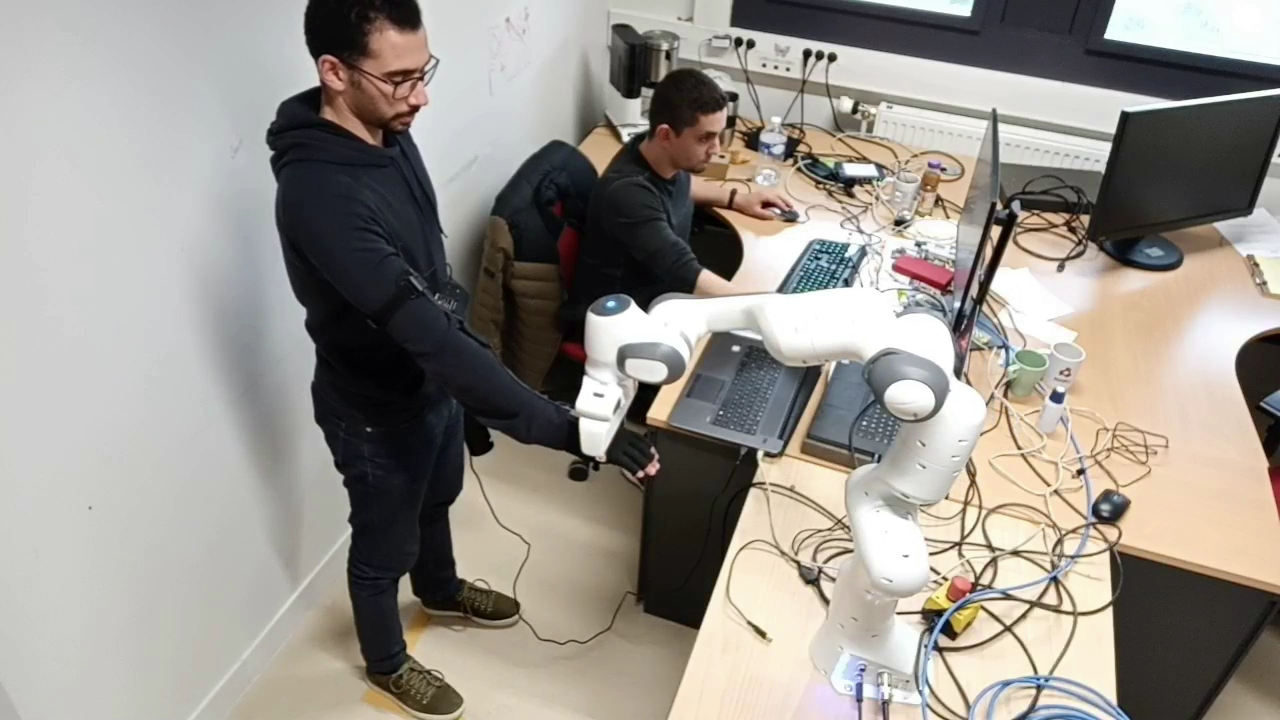
\includegraphics[width=0.4\columnwidth]{calibration}
		\caption{Calibration process.}
		\label{fig:calibration}
	\end{figure}
\begin{figure}
	\centering
	\includegraphics[width=1\columnwidth]{HOL_rm_background_initialState}%_initialState}
%\includegraphics[width=0.32\columnwidth]{HOL3_rm_background}%_initialState}
%\includegraphics[width=0.32\columnwidth]{HOL2_rm_background}%_initialState}
\caption{Different desired HOLs (red)  by the human operator where the object is a black cylindrical container. The transparent robots represent the robot initial configuration.  The IMUs are shown in \cref{fig:mocap_suit} are highlighted.}
\label{fig:HOL}
\end{figure}
\begin{figure}
\centering
\subfloat[]{
\includegraphics[width=0.492\columnwidth]{obsPosition}
\label{subfig:observation-Position}
}
\subfloat[]{
\includegraphics[width=0.492\columnwidth]{obsOrientation}
\label{subfig:observation-Orientation}
}
%\includegraphics[width=0.492\columnwidth]{obsOrientation}
\caption{Pose of the frame $\frameObj$ (dashed) from sensor and that of the  frame  $\frameObs$ (solid) obtained by the observation task. \subref{subfig:observation-Position} Cartesian coordinates. \subref{subfig:observation-Orientation} Orientation with RPY angles.}
\label{fig:obsPose}
\end{figure}
\begin{figure}
\centering
\subfloat[]{
\includegraphics[width=0.492\columnwidth]{LinVelObservation1}
\label{subfig:observation-LinVel}
}
\subfloat[]{
\includegraphics[width=0.492\columnwidth]{AngVelObservation1}
\label{subfig:observation-AngVel}
}
%\includegraphics[width=0.492\columnwidth]{obsOrientation}
\caption{Velocity of the frame $\frameObs$  obtained by the observation task. \subref{subfig:observation-LinVel} Linear velocity. \subref{subfig:observation-AngVel} Angular velocity. }
\label{fig:obsVel}
\end{figure}
\begin{figure}
\centering
\subfloat[]{
\includegraphics[width=0.492\columnwidth]{LinAccObservation1}
\label{subfig:observation-LinAcc}
}
\subfloat[]{
\includegraphics[width=0.492\columnwidth]{AngAccObservation1}
\label{subfig:observation-AngAcc}
}
%\includegraphics[width=0.492\columnwidth]{obsOrientation}
\caption{Acceleration of the frame $\frameObs$  obtained by the observation task. \subref{subfig:observation-LinAcc} Linear acceleration. \subref{subfig:observation-AngAcc} Angular acceleration. }
\label{fig:obsAcc}
\end{figure}
	\subsection{Multi-Tasks QP Formulation}
	This subsection shows how the tasks and constraints discussed above are combined using a multi-objective and multi-robots QP formulation. 
	Let us extend the decision variables vector $\decisionVector$ in \cref{eq:decision variables vector} to consider the object as a second robot
	\begin{equation}
		\decisionVector=\begin{bmatrix}
			\genActConfDDot \\ \obsPoseDDot \\ \force
		\end{bmatrix}\in\mathbb{R}^{n+15}
	\end{equation} 
	 %the vector encompassing the linear and angular acceleration of the observed rigid-body object, the joint-acceleration of the robotic arm, and the contact force.
	Given the affinity of \cref{eq:mu observartion task} w.r.t $\obsPoseDDot$,  that of \cref{eq:mu grasping-point-tracking task,eq:mu segline track task,eq:mu grasping-set constraint,eq:mu posture task} w.r.t $\genActConfDDot$, and that of \cref{eq-chap0:equation of motion} w.r.t $\genActConfDDot$ and $\force$,  we can combine all the tasks and constraints in a single weighted-prioritized QP formulation 
	\begin{subequations}\label{eq:QP formulation handover}
		\begin{align}
			\label{eq:QP cost-function}\underset{\chi}{\min} &\sum_{i}w_i\norm{\mathbf{G}^i\decisionVector+ \bm{g}^i}^2 \\
			\label{eq:QP constraint}\text{S.t:~} &\mathbf{A}_{\rm ineq}\decisionVector\leq \bm{b}_{\rm ineq}
		\end{align}
	\end{subequations}
	where $w_i>0$ is the associated weight to each task $i$.
	The main advantage of QP formulation~\eqref{eq:QP formulation handover} is its \emph{compactness}: enables handling multi-robot control. The robotic arm and the object are considered as two distinct robots entities. This allows adding other robots to achieve the handover (e.g., bi-arm handover) while still using one compact formulation~\cite{bouyarmane2019tro}. This property shall be shown in the next experimental section.
%	\begin{itemize}
%		\item \emph{Mediation:} combine the different competing tasks in~\eqref{eq:QP cost-function} by settling a soft prioritization scheme;
%		\item \emph{Unilateral constraints:} embed limitations like joint-position, velocity, acceleration and torque limits, (self-)collision avoidance... in~\eqref{eq:QP constraint}~\cite{djeha2020ral};
%		\item \emph{Joint-space mapping:} seeks optimal $\ddot{q}$ that generates the robotic arm motion that achieve \emph{at best} all the tasks while fulfilling all the constraints;
%		\item \emph{Compactness:} enables handling multi-robot control. The robotic arm and the object are considered as two distinct robots entities which opens the possibility to add other robots to achieve the handover (e.g., bi-arm handover) while still using one compact formulation~\cite{bouyarmane2019tro}.
%	\end{itemize}

%	QP~\eqref{eq:QP formulation} is constructed and solved at each iteration. $\ddot{q}$ in $\chi$ is integrated twice to obtain the desired joint velocity $\dot{q}$ and position $q$ which are sent to the joint-level robot controller as command inputs. 
%	\begin{figure}[t!]
%		\centering
%		\subfloat[]{
%			\includegraphics[width=0.45\columnwidth]{cuboid_object_SymmetryAxis2}
%			%	\caption{Cuboid object with attached frames $\setR_{\rm obs}$ and $\setR_{\rm grasp}$ in addition to the unit orthogonal vectors $u_{\rm grasp}$ and $n_{\rm grasp}$.}
%			\label{subfig:cuboid_object}}
%		\subfloat[]{
%			\includegraphics[width=0.45\columnwidth]{Cylinder_object_SymmetryAxis3}
%			%	\caption{Cuboid object with attached frames $\setR_{\rm obs}$ and $\setR_{\rm grasp}$ in addition to the unit orthogonal vectors $u_{\rm grasp}$ and $n_{\rm grasp}$.}
%			\label{subfig:cylinder_object}}
%		\hfil
%		\subfloat[]{
%			\includegraphics[width=0.45\columnwidth]{end-effector_axis3}
%			\label{subfig:end-effector}}
%		\caption{Different handover objects (\subref{subfig:cuboid_object} cuboid object,~\subref{subfig:cylinder_object} cylindrical object) with the attached frames $\frameObs$ and $\frameGrasp$ as well as the end-effector (\subref{subfig:end-effector} Panda gripper) with attached frame $\frameEndEff$. The colored vectors in $\frameEndEff$ tracks the same orientation of their corresponding ones in $\frameGrasp$. For the cylindrical object, only the yellow  vector needs to be aligned.}
%		\label{fig:handover objects}
%	\end{figure}

\section{Experimental Result}\label{sec-chap4:experiments} 
For demonstration, we implemented our approach on the open-source code implementation of the QP controller interface \mcrtc.~% that includes user task-specification interface, debugging, data recording for both simulation and real-time control. 
Based on the embedded sensors data, \mcrtc~builds and solves the QP problem at each control cycle (1~ms). Experiments are conducted using 7-DoF robotic arm Panda from Franka-Emika. 

Perception Neuron\footnote{\url{https://neuronmocap.com/}} sensor-suit has been used for the pose measurement. An API provides the hand pose in a given fixed frame at a frequency of 60~Hz. The sensor suite has been mounted on the human left arm as shown in  \cref{fig:mocap_suit}. A calibration step is necessary to correctly coincide the sensor frame with the controller world-frame. It consisted of putting the left-hand sensor on the Panda end-effector frame $\frameEndEff$. Then, the offset between $\objPose$ and $\endEffPose$ is removed manually to have $\objPose=\endEffPose$ (\cref{fig:calibration}). The calibration process is repeated at the beginning of each handover experiment to avoid drifting.    
A ROS node has been implemented to handle the data streaming between the API and the controller.  
When the human is a giver, the object is assumed to be rigidly attached to the hand, and thereby its pose $\objPose$ can be computed based on the hand's one.
%After a calibration step, the measured object pose $X_{\rm {obj}}$ in~\eqref{eq:object pose} is given as a reference for the observation task as shown in \cref{subsec:observation task}.


Several handover scenarios have been performed where the robot starts from different configurations. In addition, multiple HOLs have been tried (\cref{fig:HOL}). The objects used during experiments are a small cylindrical container and a small cuboid object made with a carton. The implemented tasks are the observation task (\cref{subsec-chap4:observation task}) and trajectory tracking task (\cref{subsec-chap4:trajectory tracking}).




%\begin{figure}
%	\centering
%	\includegraphics[width=0.32\columnwidth]{HOL1_rm_background}%_initialState}
%	\includegraphics[width=0.32\columnwidth]{HOL3_rm_background}%_initialState}
%	\includegraphics[width=0.32\columnwidth]{HOL2_rm_background}%_initialState}
%	\caption{Different HOLs (red) desired by the human operator where the object is black cylindrical container. The IMUs shown in \cref{fig:mocap_suit} are highlighted.}
%	\label{fig:HOL}
%\end{figure}


The observation task gains have been set to high values $\mathbf{K}_{\rm{s}}^{\rm obs} = 1500\mathbf{I}$, and  $ \mathbf{K}_{\rm d}^{\rm obs} = 2\sqrt{\mathbf{K}_{\rm{s}}^{\rm obs}}$ to track accurately the object pose $\objPose$, and generate a good estimation $\bm{s}_{\rm obs}$ in \cref{eq:observer full-state} of the object full state $\bm{s}_{\rm obj}$ \cref{eq:object full-state}.  \cref{fig:obsPose} shows how $\obsPose$ tracks $\objPose$. Even though the latter is varying, the high observation task gains allows an accurate pose tracking. In the same, it allows to a good estimation of $\objPoseDot$ and $\objPoseDDot$ by computing $\obsPoseDot$ and $\obsPoseDDot$ from \cref{eq:observation-task closed-loop} (see \cref{fig:obsVel} and \cref{fig:obsAcc}). 



%\begin{figure}
%	\centering
%	\includegraphics[width=1\columnwidth]{HOL}
%	\caption{Different HOLs desired by the human operator where the object is black cylindrical container.}
%	\label{fig:HOL}
%\end{figure}



Consequently, $\bm{s}_{\rm obs}$ in \cref{eq:observer full-state} is fully constructed, which allows implementing the trajectory tracking for the end-effector to meet the object. 
Given $\obsPose$, the frame $\graspPose$ is specified such that $\graspPosition^{{\rm grasp}^{\tp}} = \begin{bmatrix} 0.07& 0.00& 0.03 \end{bmatrix}$. $\graspPosition$ is then computed from \cref{eq:forward position}. 
Then, the trajectory-tracking task is formulated as described in \cref{subsec-chap4:trajectory tracking} where the gains are fixed as $\mathbf{K}^{\rm tt}_{\rm s} = \begin{bmatrix}
	\mathbf{I} & \mathbf{0}\\\mathbf{0} & 2\mathbf{I}
\end{bmatrix}$ and $\mathbf{K}^{\rm tt}_{\rm d} = \begin{bmatrix}
	2\sqrt{\mathbf{I}} & \mathbf{0}\\\mathbf{0} & 2\sqrt{2\mathbf{I}}
\end{bmatrix}$. The orientation stiffness has been chosen to be twice bigger than those of the translation to ensure that  end-effector reaches the object while its orientation has already converged to the target. This also implies that the orientation is tracked better than the position as it can be observed from \cref{fig:trajTrack}. Furthermore, the object and the end-effector meet seamlessly and smoothly at the HOL without being specified in prior as it can be seen from the 3D trajectories of the grasping frame $\frameGrasp$ and the end-effector frame $\frameEndEff$ in \cref{fig:3D plot}. %Furthermore, the end-effectors adapts reactively to the variation of the grasping point.
\begin{figure}
	\centering		
	\subfloat[]{
		\includegraphics[width=0.492\columnwidth]{surfPosition}
		\label{subfig:trajTrack-Position}
	}
	\subfloat[]{
		\includegraphics[width=0.492\columnwidth]{surfOrientation}
		\label{subfig:trajTrack-Orientation}
	}
	\caption{Pose of the frame $\frameGrasp$ (dashed) and that of the frame $\frameEndEff$ (solid) obtained by the trajectory-tracking task. \subref{subfig:trajTrack-Position} Cartesian coordinates. \subref{subfig:trajTrack-Orientation} Orientation with RPY angles. The sudden variation in the yaw angle is sound because the angle is bounded between $-\pi$ and $\pi$. This does not induce any singularity issue since the orientation task is implemented using unit quaternions.}
	\label{fig:trajTrack}
\end{figure}
\begin{figure}
	\centering
	\includegraphics[width=0.6\columnwidth]{3D-2}
	\caption{3-D trajectories of the frames $\frameGrasp$ (blue) and $\frameEndEff$ (orange). The initial and terminal points are denoted with a square and a circle, respectively.  }
	\label{fig:3D plot}
\end{figure}

Next, we extended our handover QP controller to the case of multi-robot handover. In particular, we considered the case where the object is long enough so that two Panda robots are necessary to receive and safely achieve the handover. QP~\eqref{eq:QP formulation handover} is formulated by considering the two Panda and the object as three different robots.   For this purpose, we have run simulations using Matlab-Simulink. Simscape has been used to model the robots. This time, we do not specify a specific grasping point. Instead, the grasping-set-tracking task described in \cref{subsec-chap4:grasping-set-tracking} is formulated for each robot. Successive snapshots of the simulation are shown in \cref{fig:multi-robot handover}. 
\begin{figure}
	\centering
	\subfloat[$t=0$~s]{
		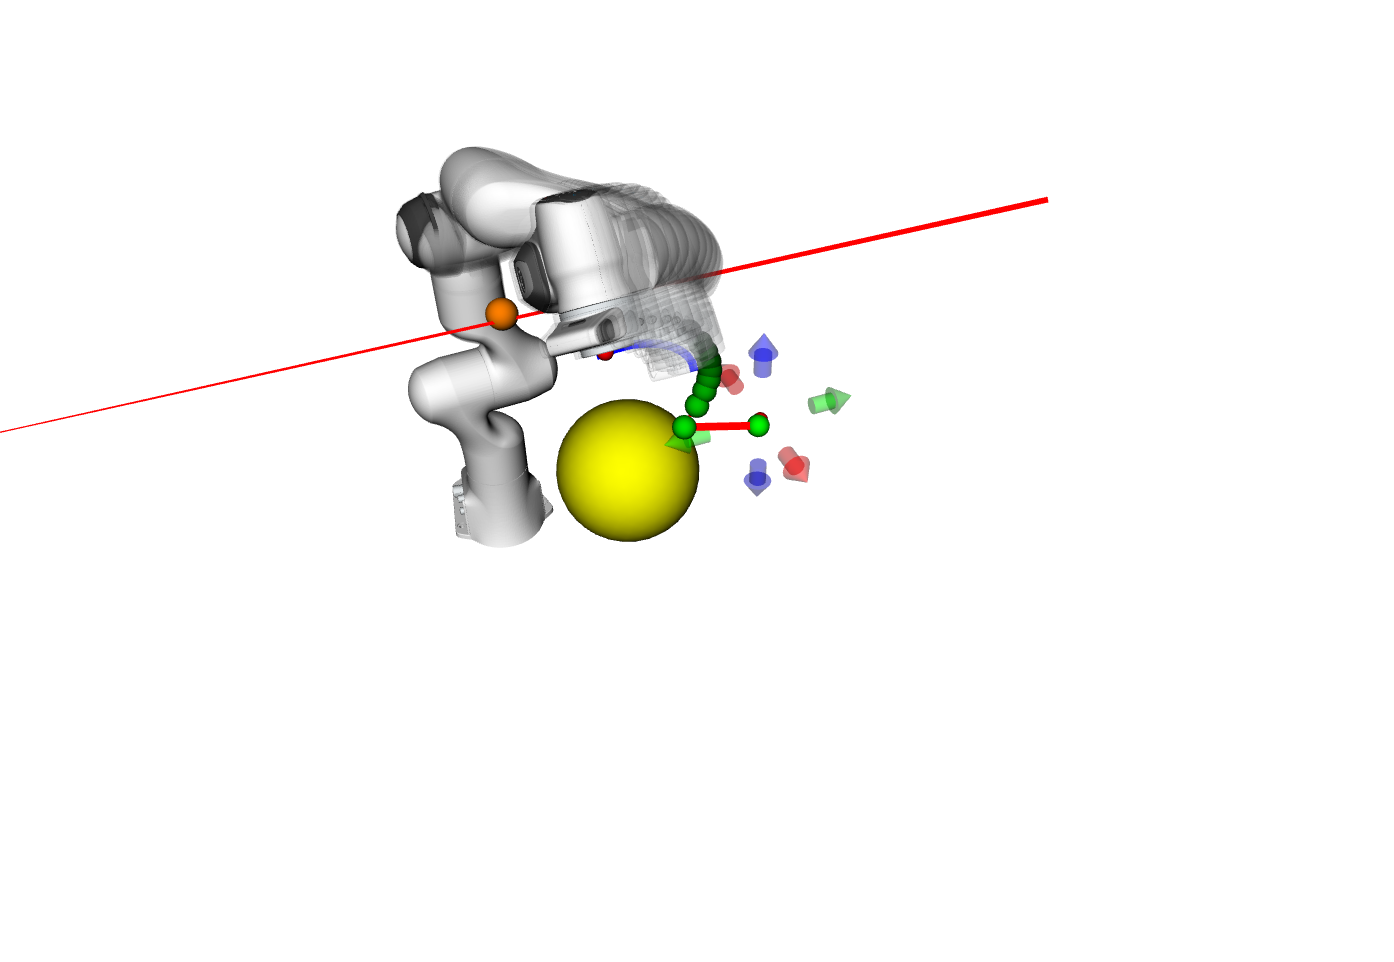
\includegraphics[width=0.32\columnwidth]{1}
	}
	\subfloat[$t=1$~s]{
		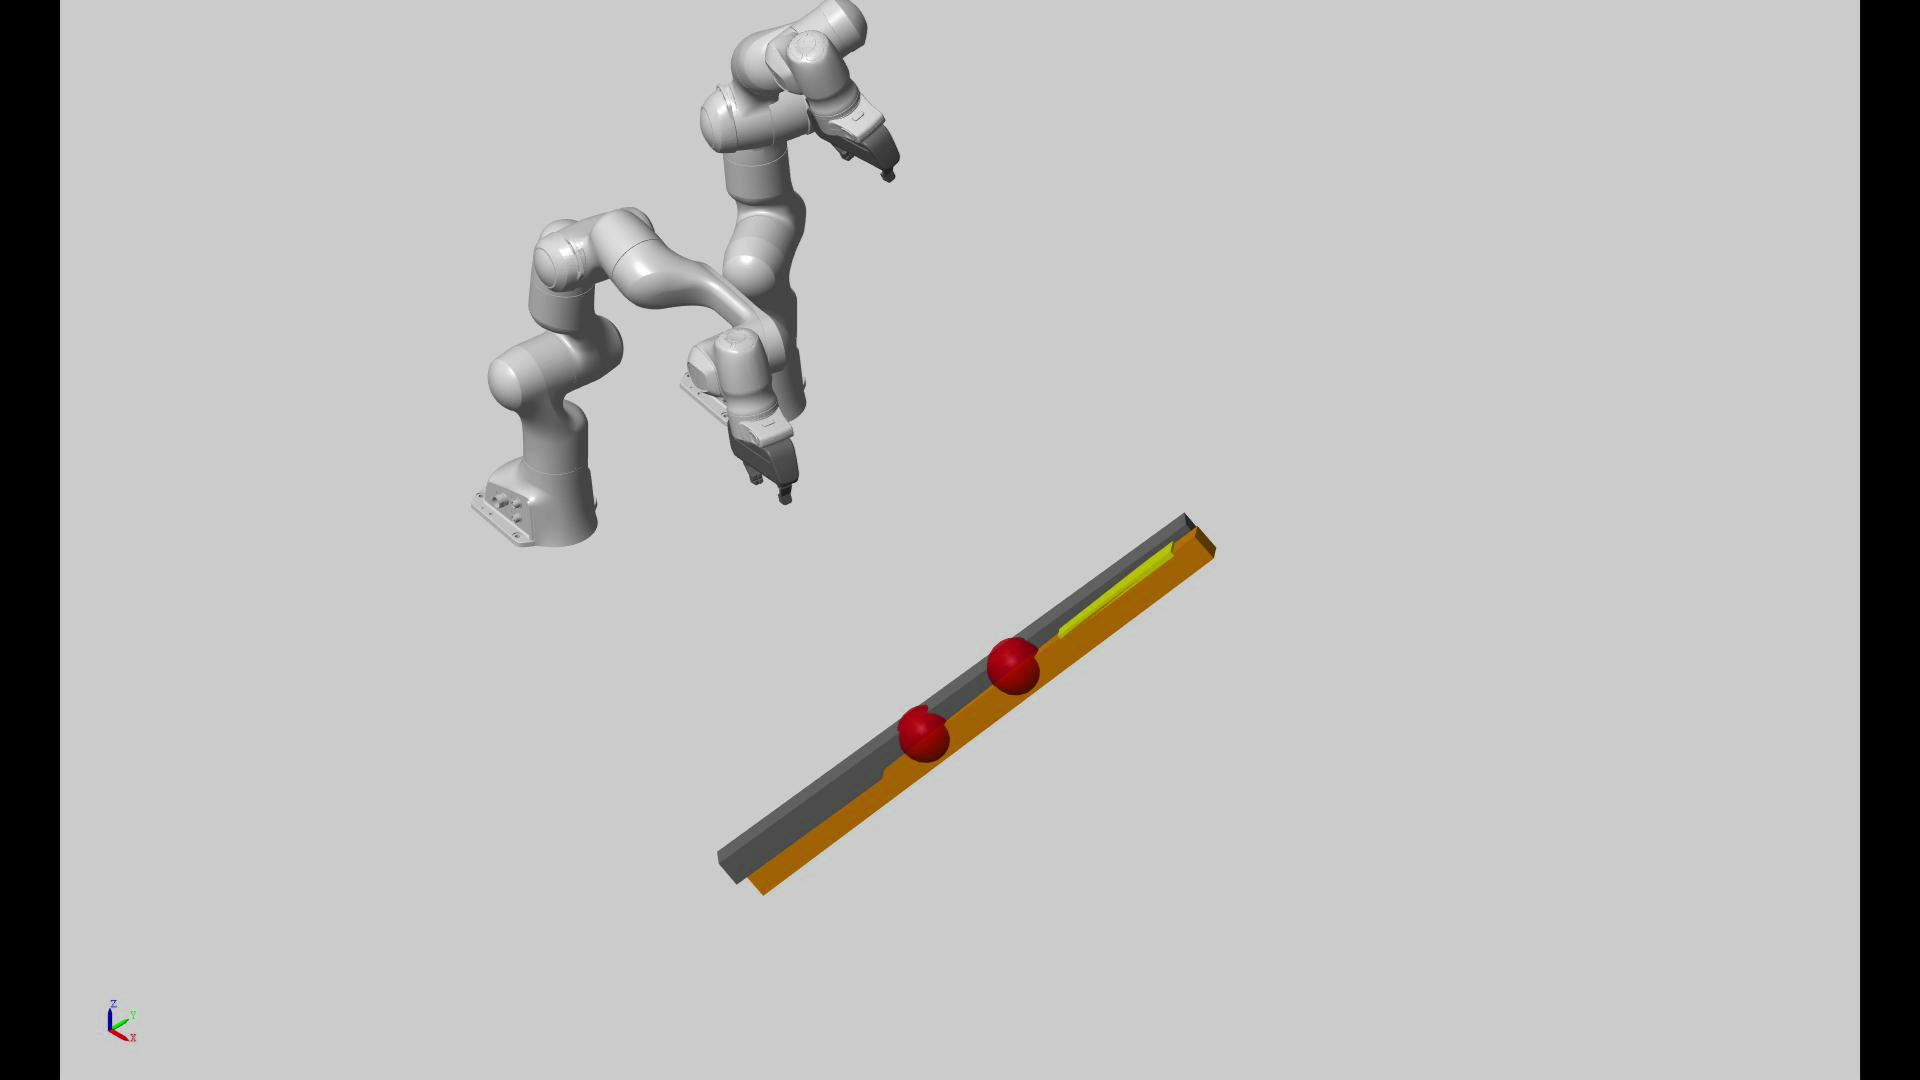
\includegraphics[width=0.32\columnwidth]{2}
	}
	\subfloat[$t=2$~s]{
		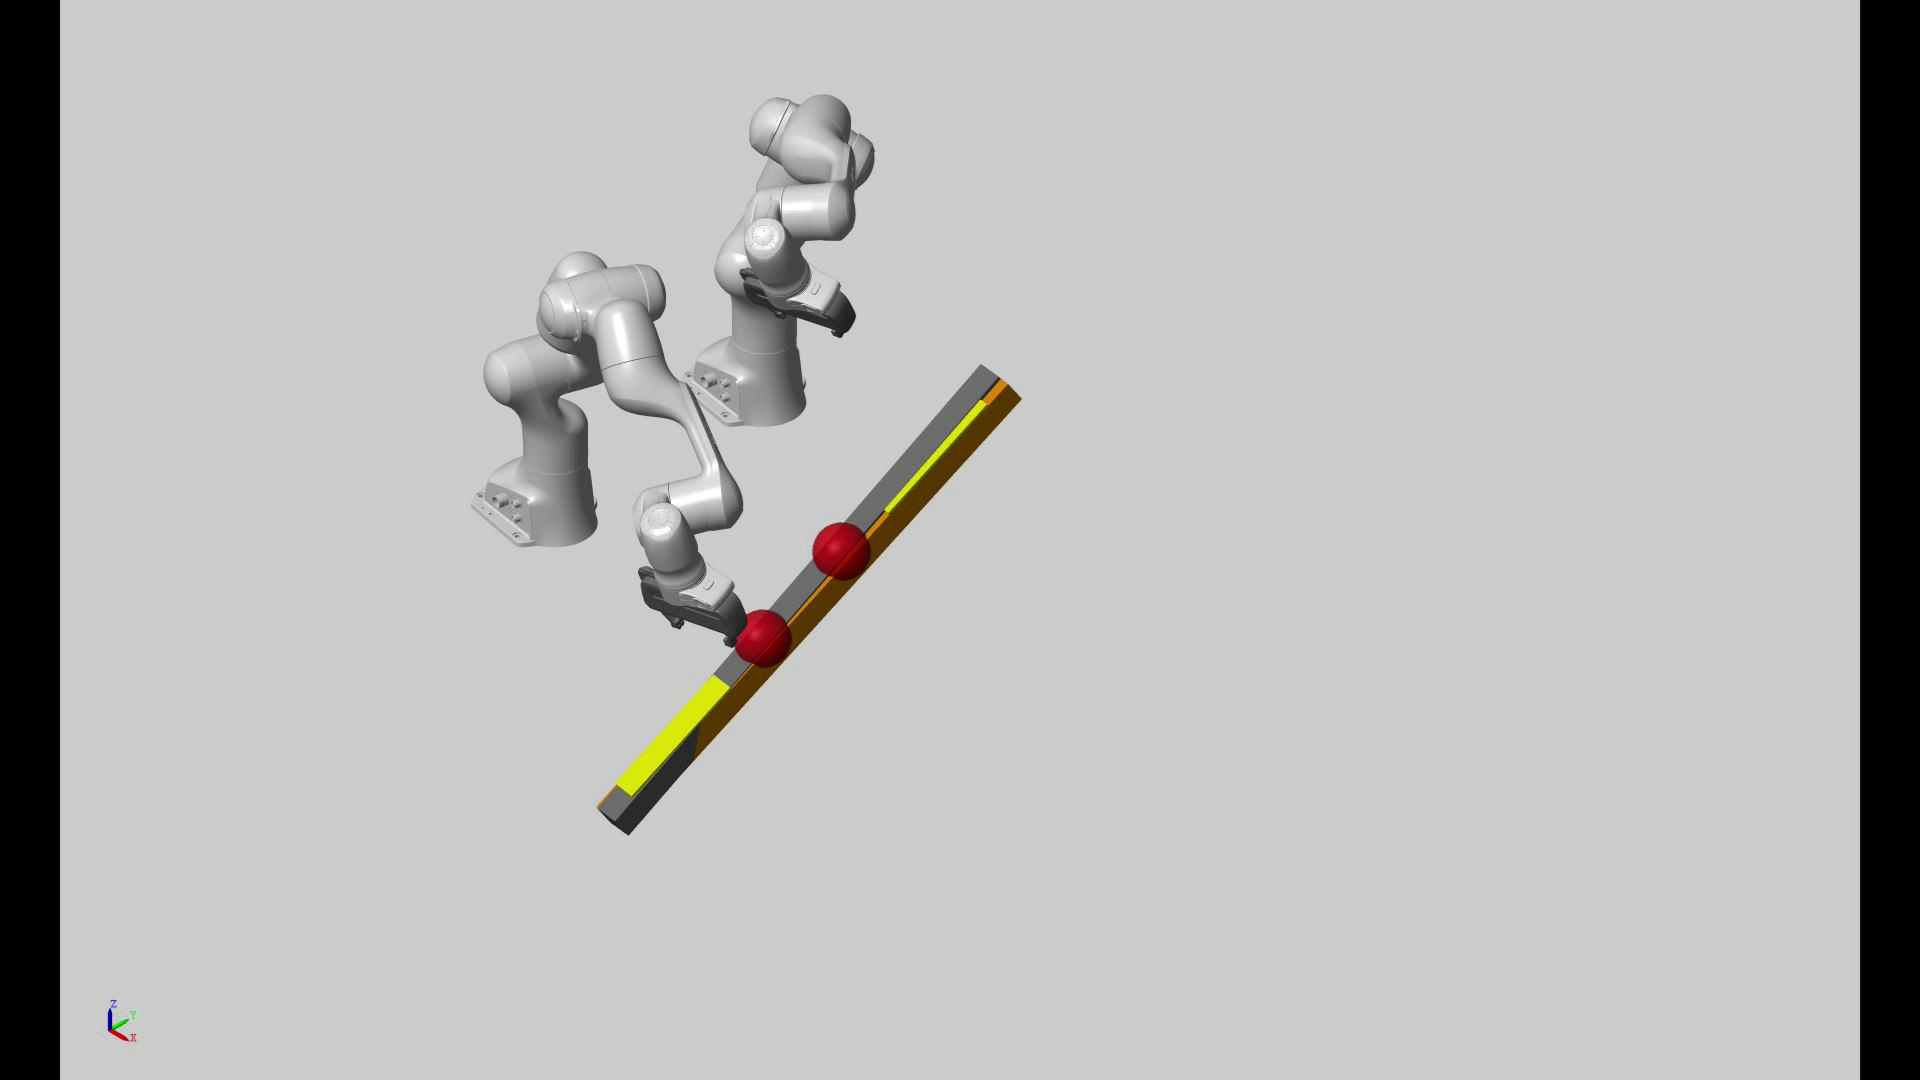
\includegraphics[width=0.32\columnwidth]{3}
	}
	\hfil
	\subfloat[$t=3$~s]{
		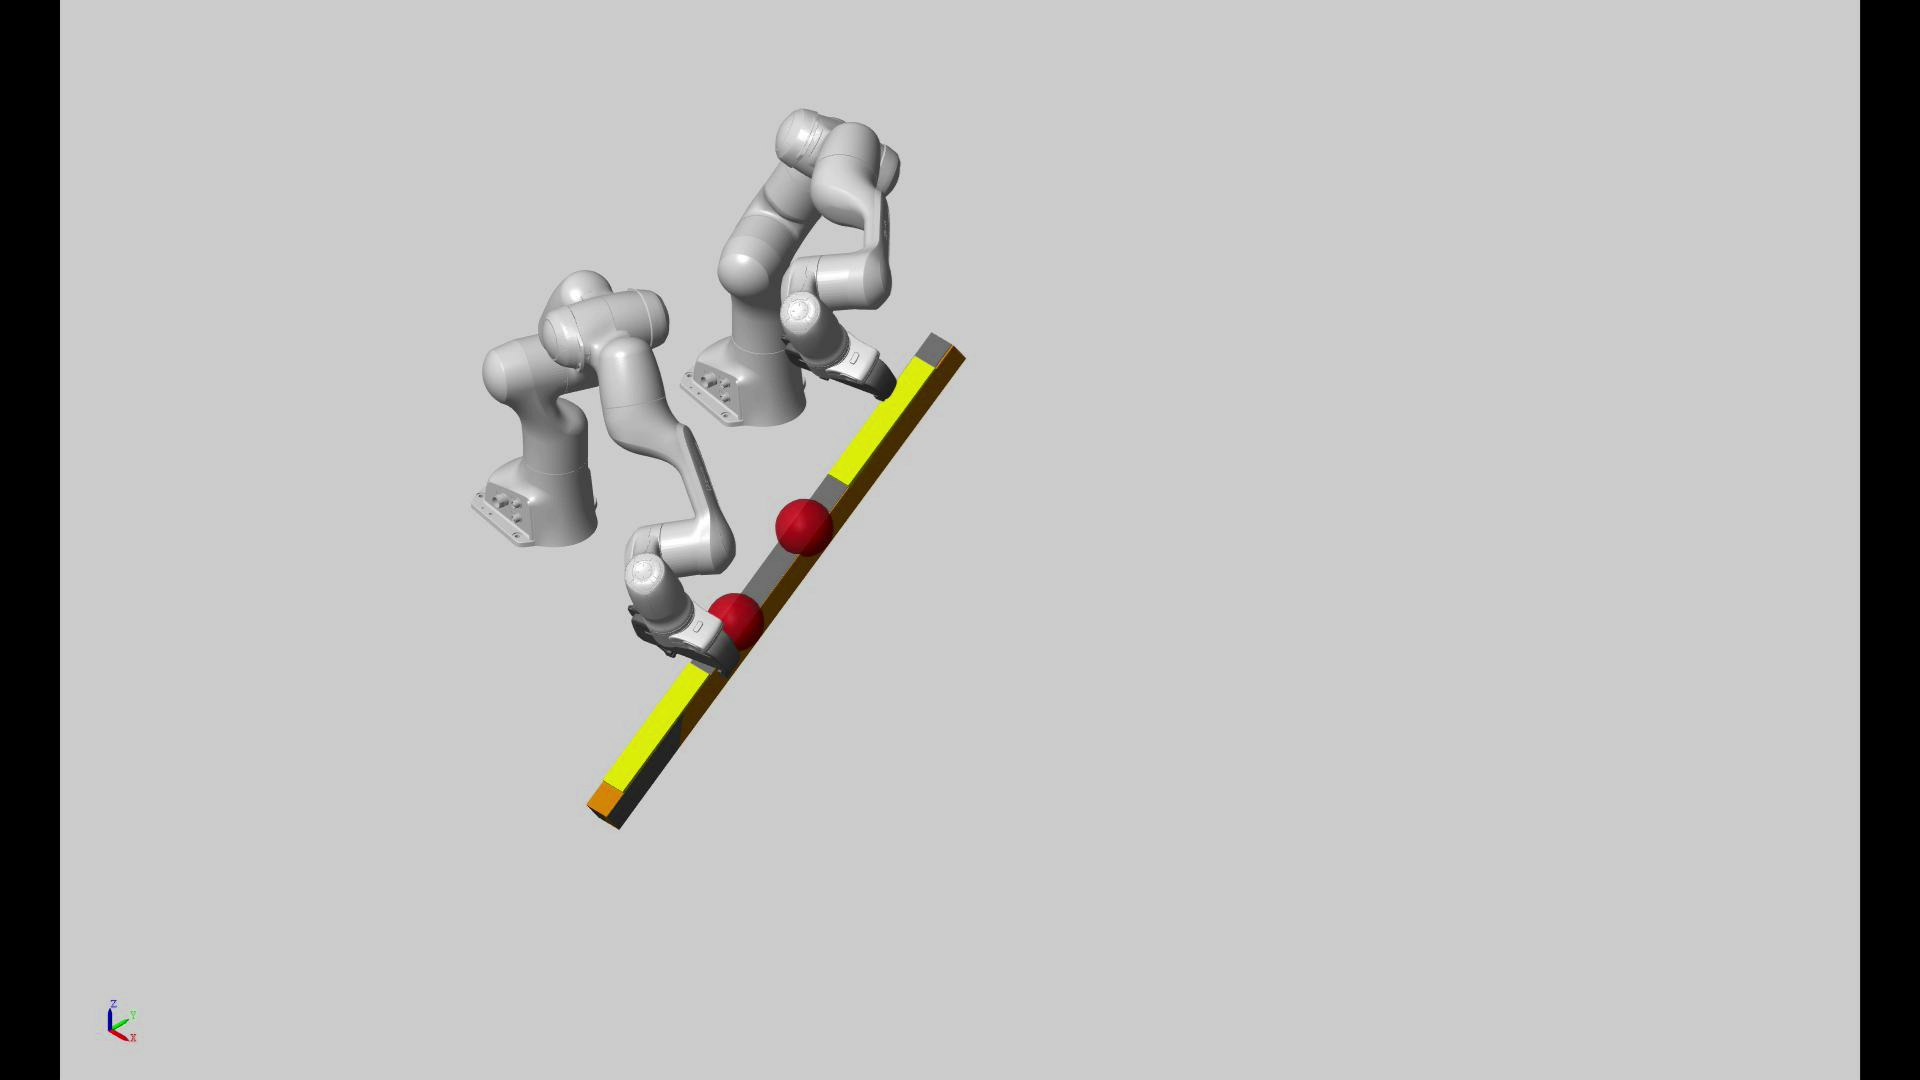
\includegraphics[width=0.32\columnwidth]{4}
	}
	\subfloat[$t=4$~s]{
		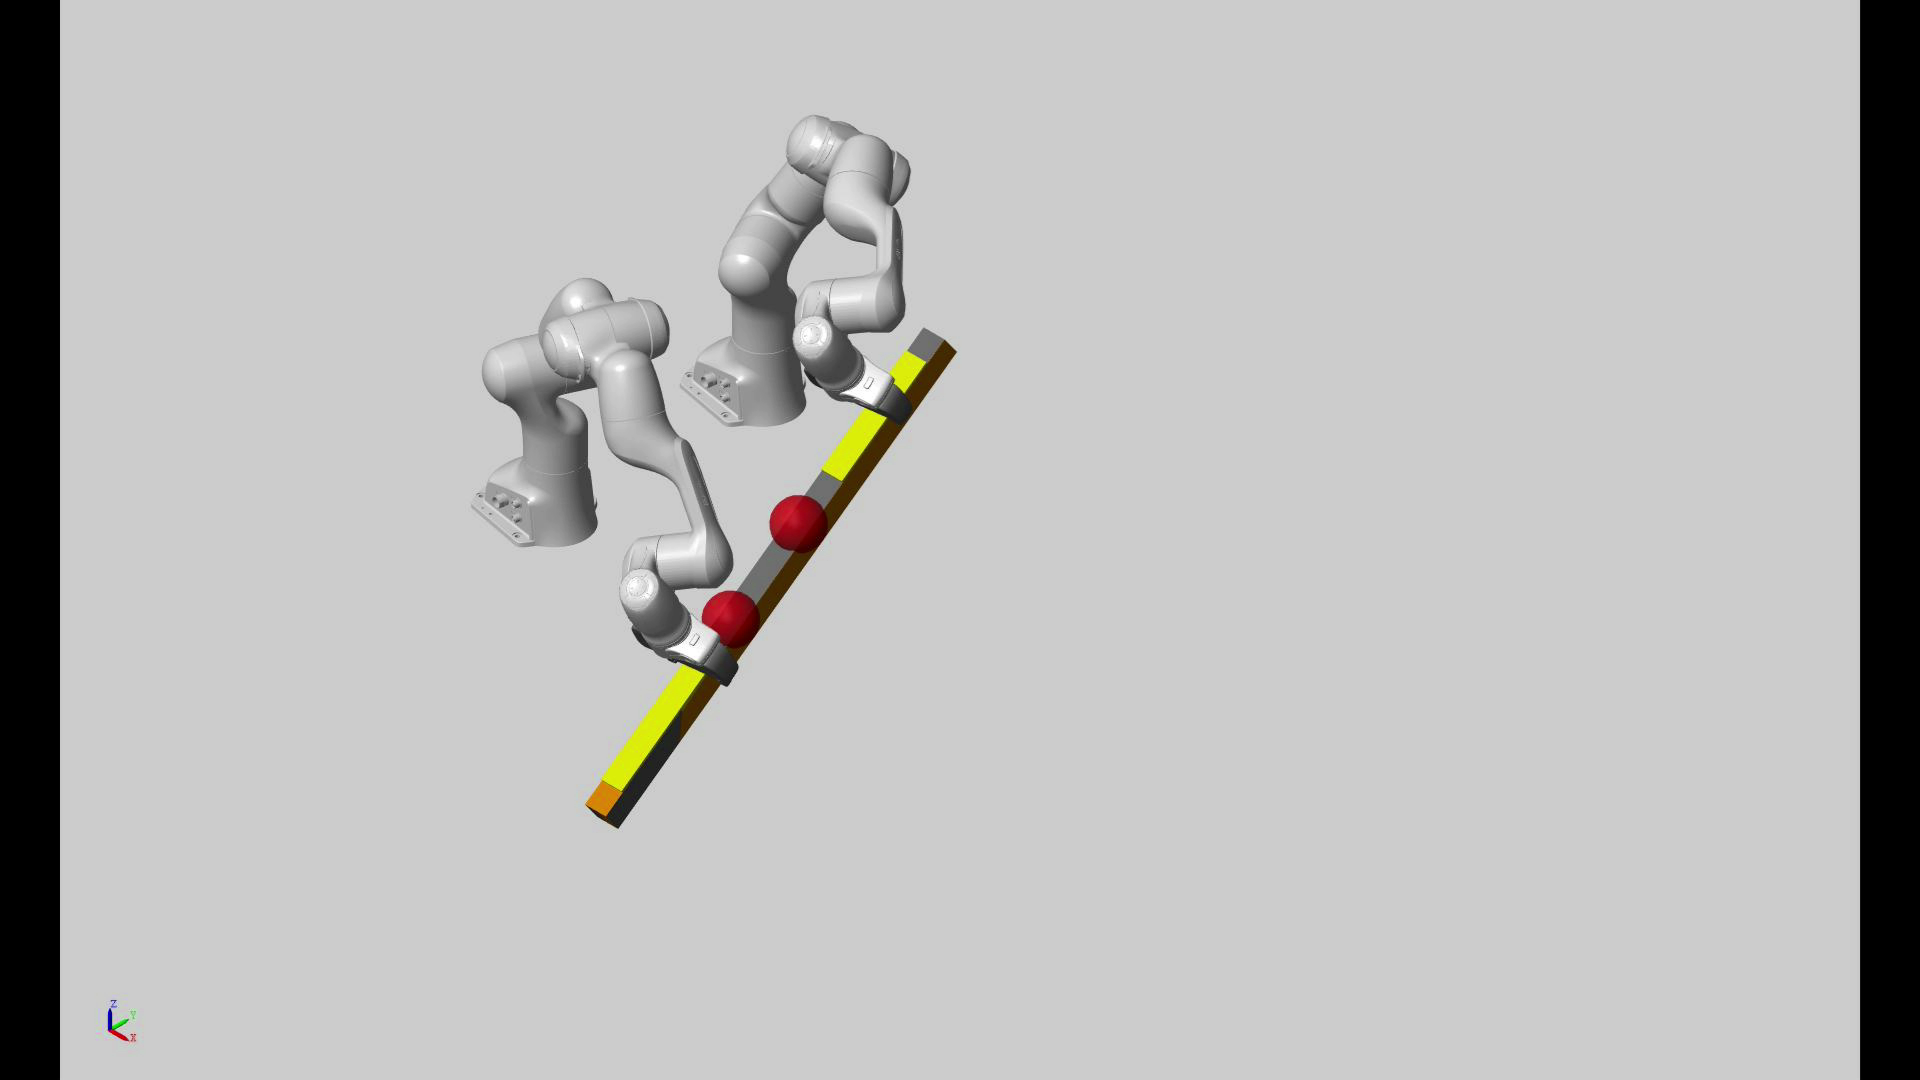
\includegraphics[width=0.32\columnwidth]{5}
	}
	\subfloat[$t=5$~s]{
		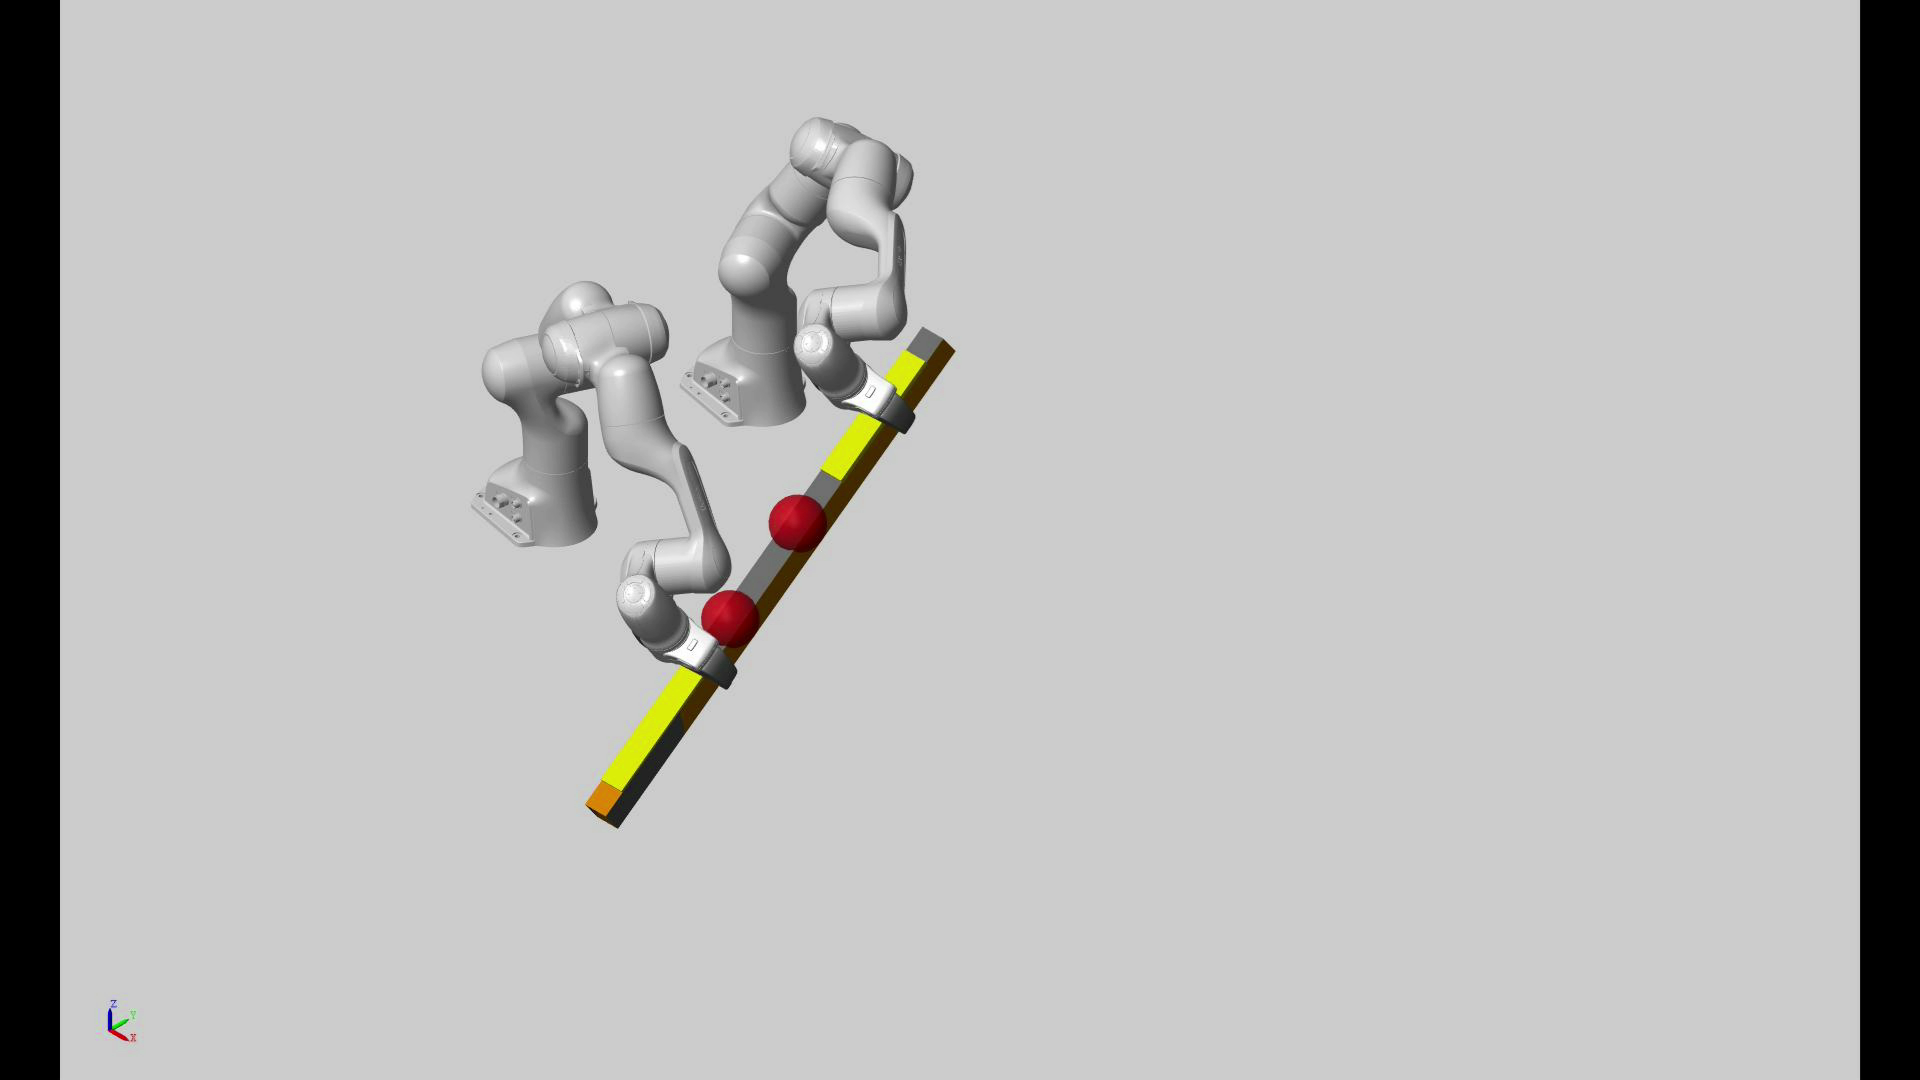
\includegraphics[width=0.32\columnwidth]{6}
	}
	%	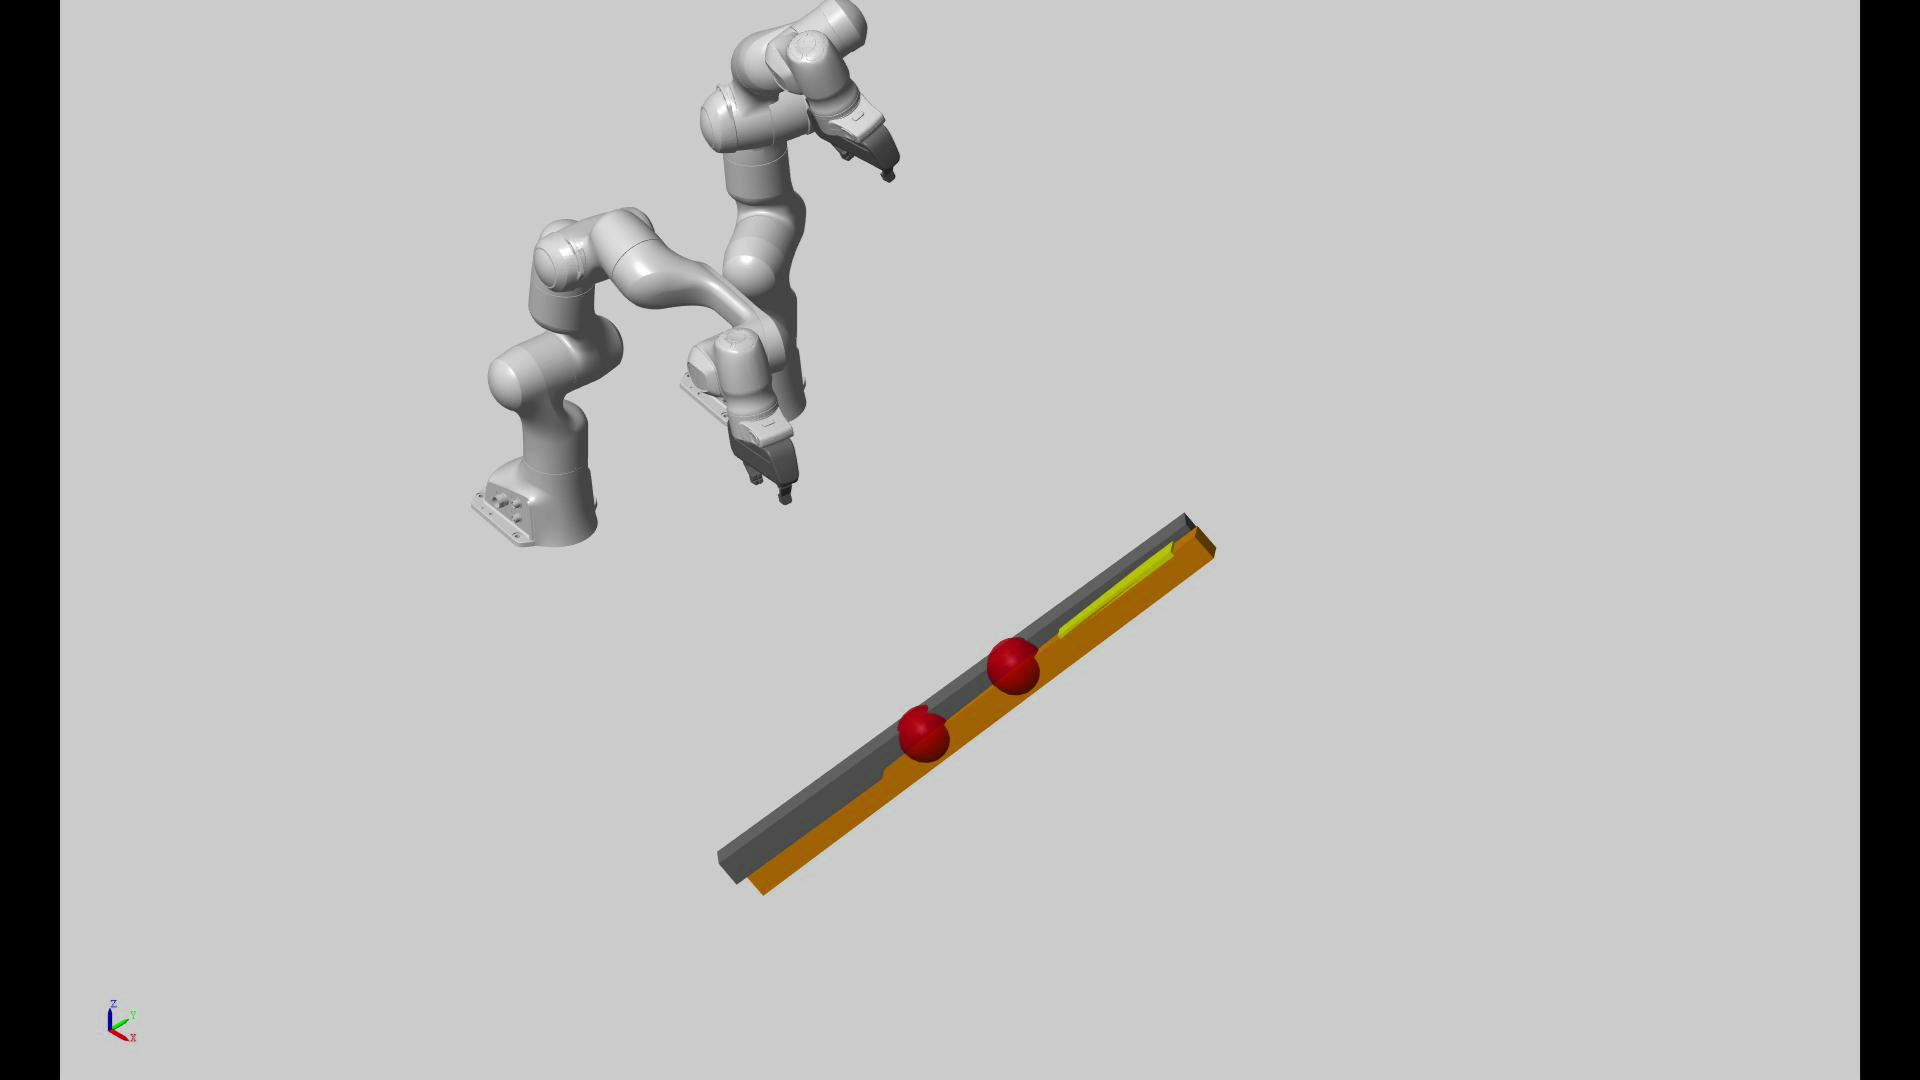
\includegraphics[width=0.32\columnwidth]{2}
	%	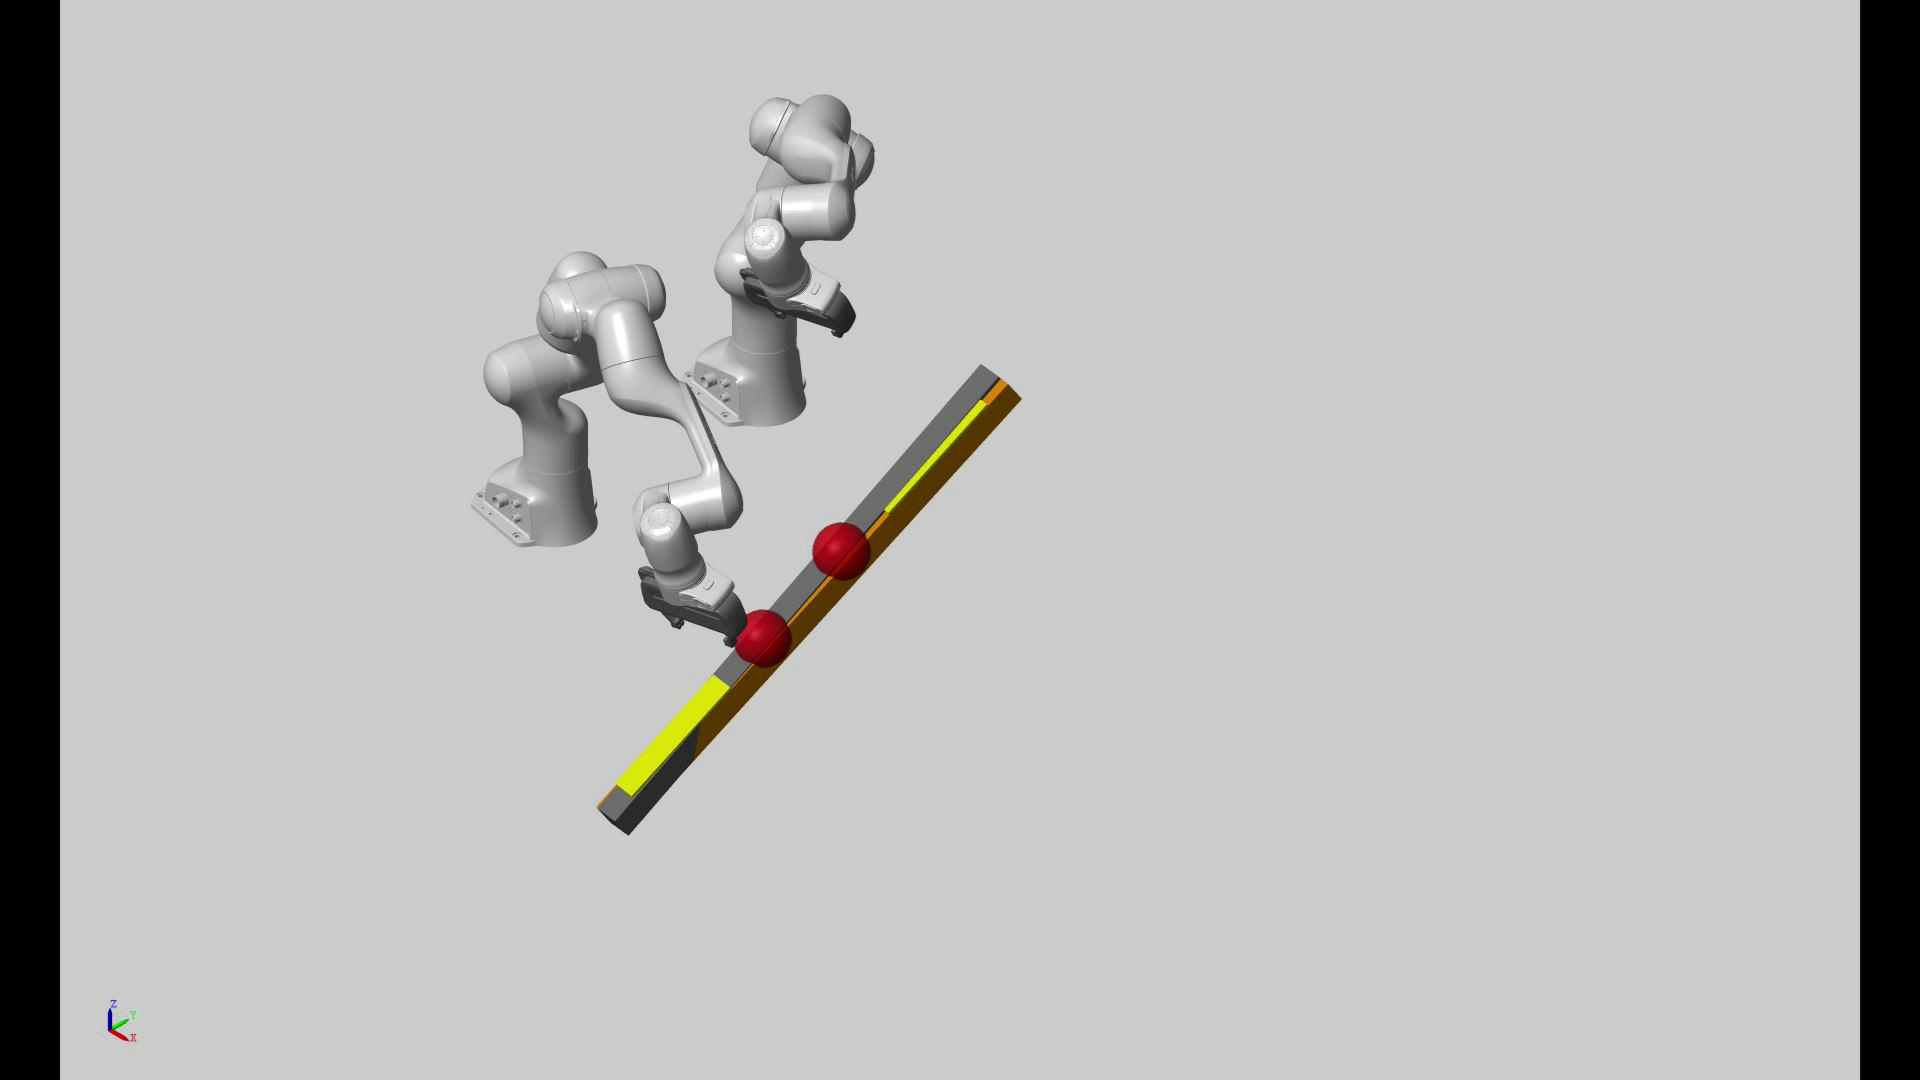
\includegraphics[width=0.32\columnwidth]{3} \\
	%	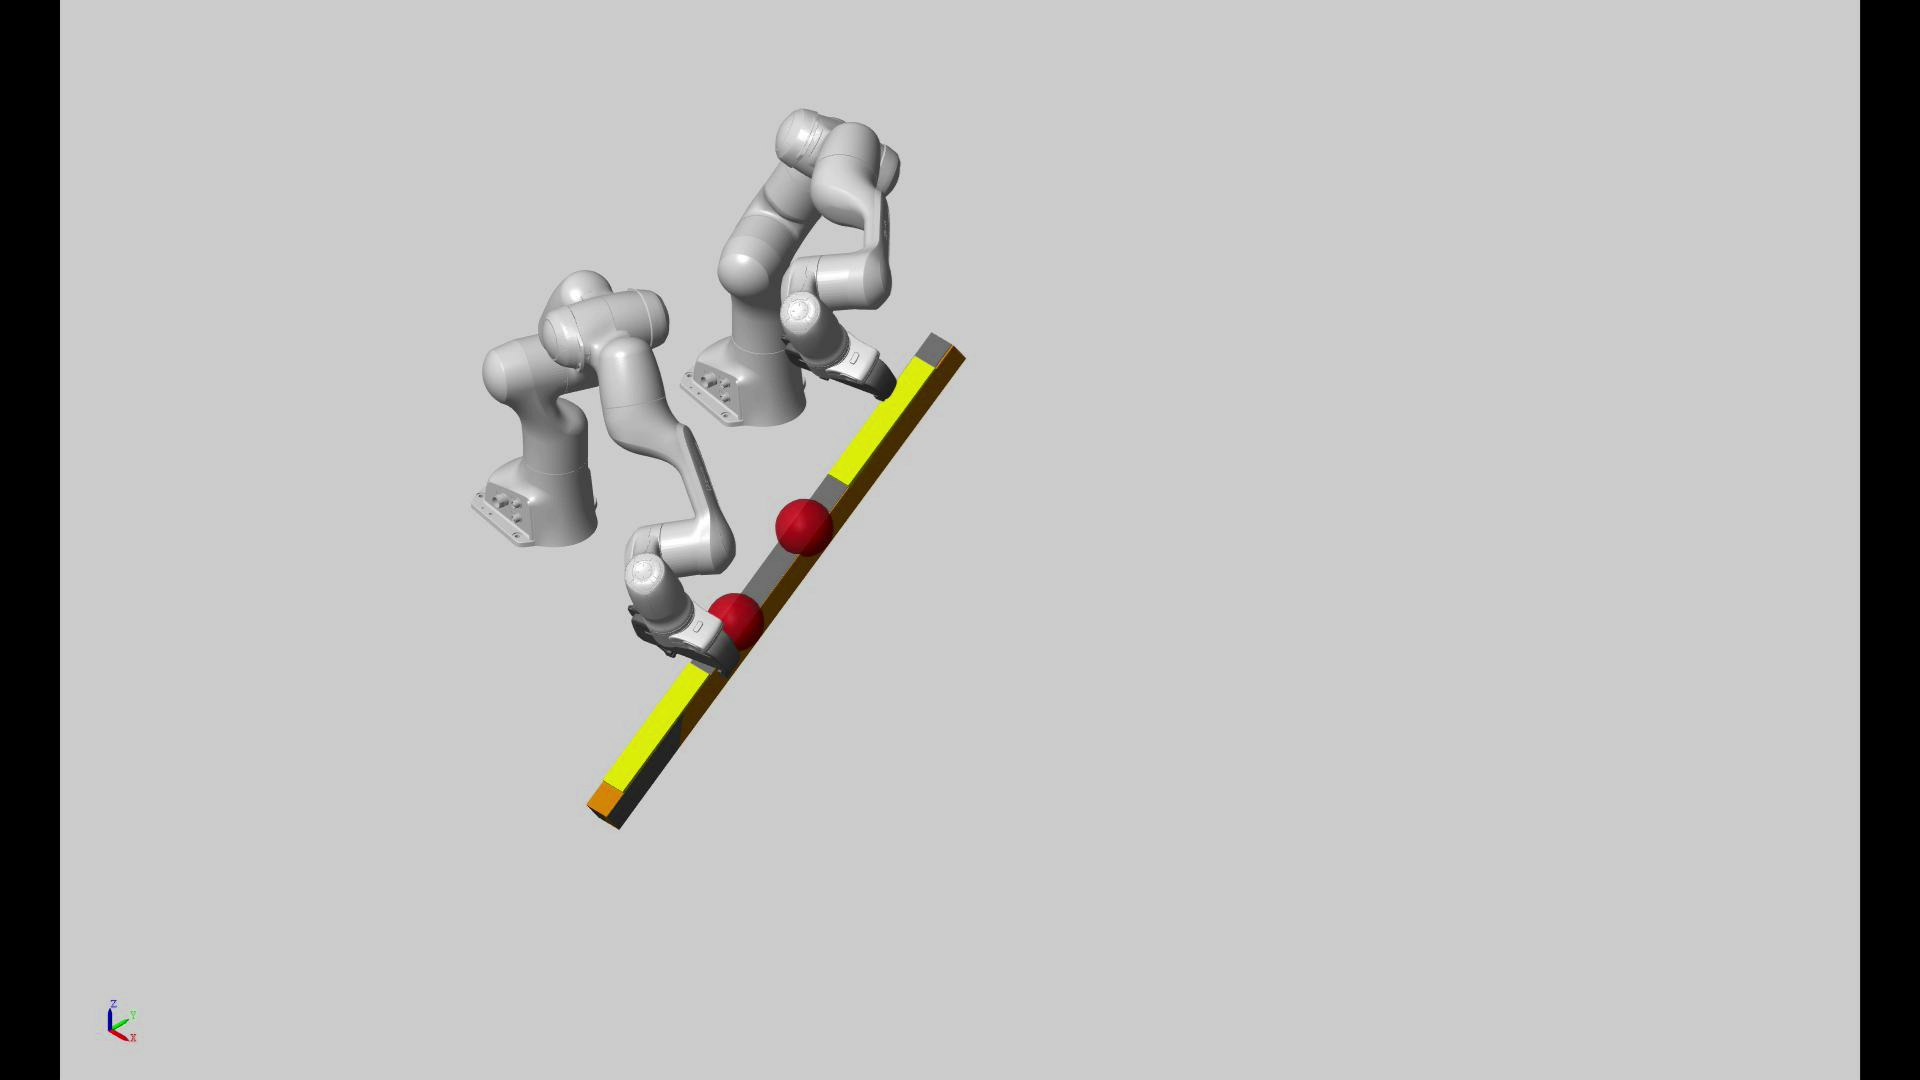
\includegraphics[width=0.32\columnwidth]{4}
	%	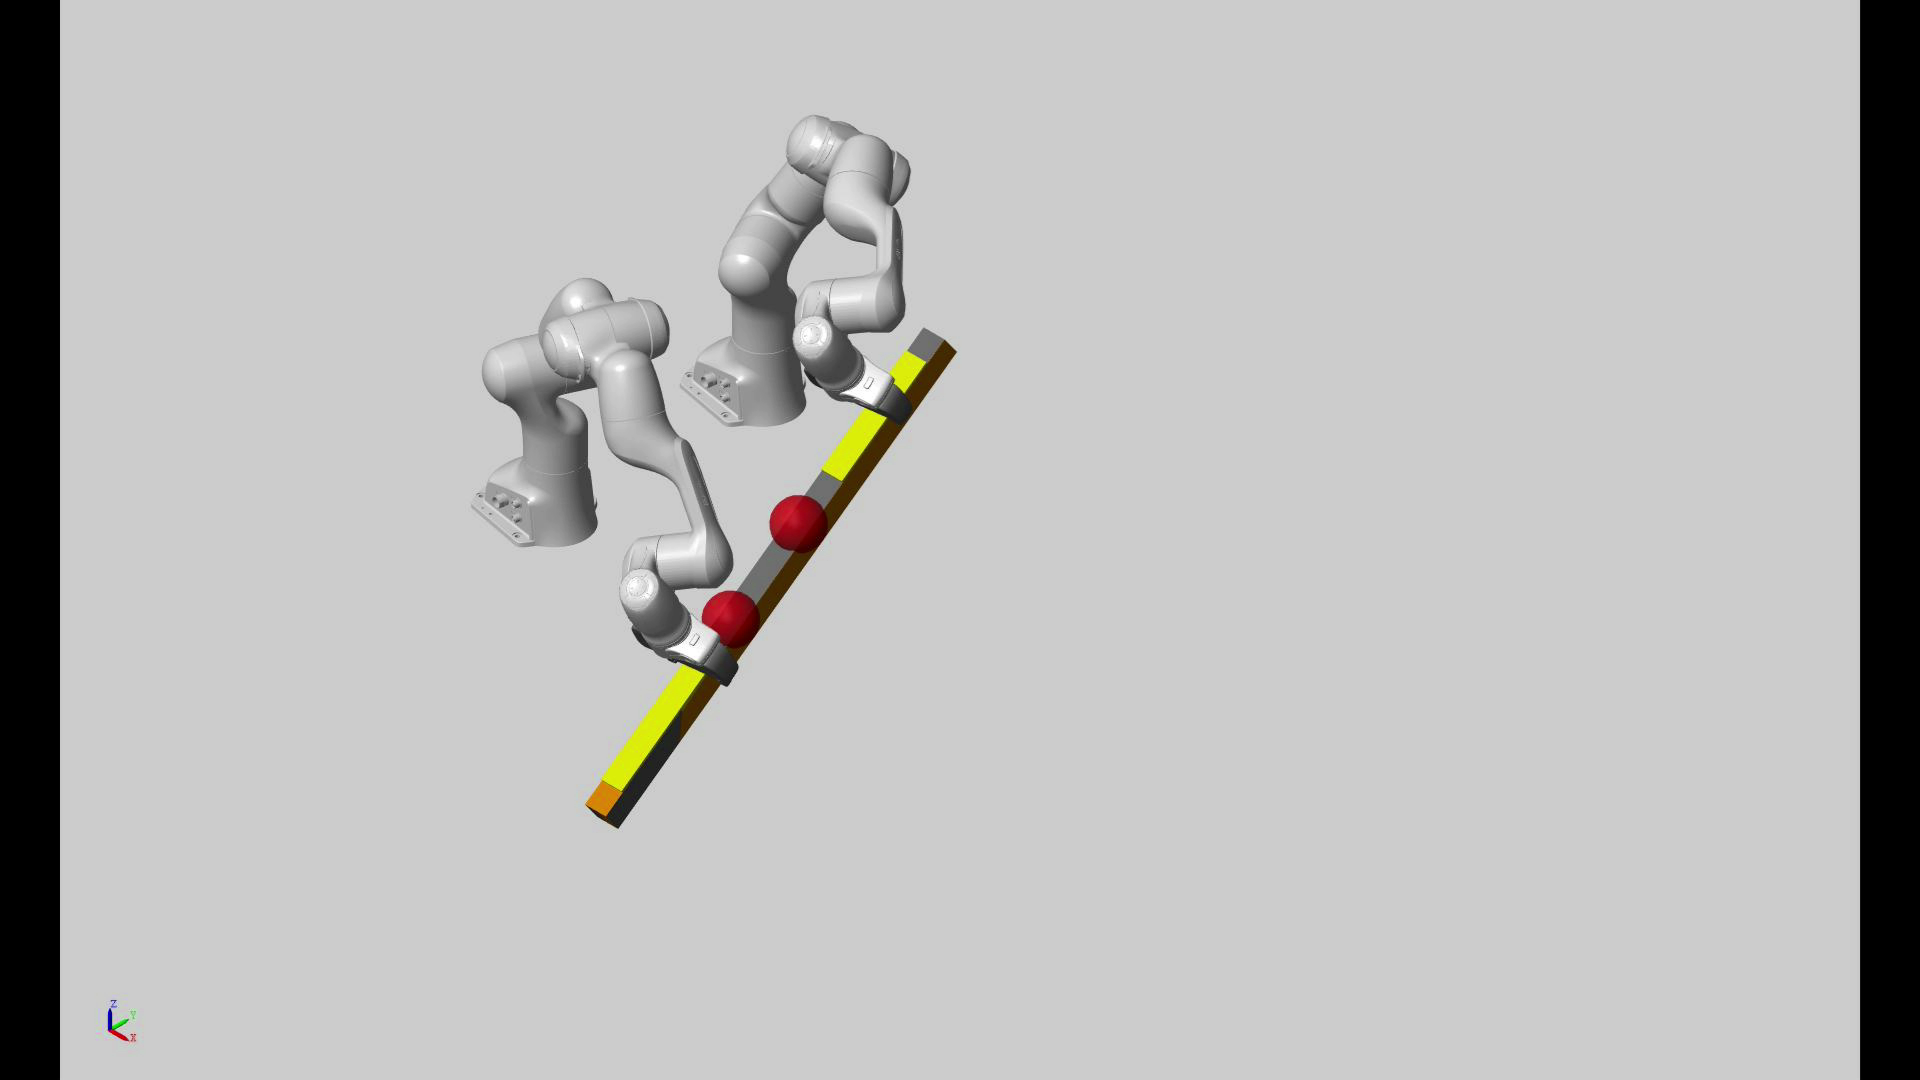
\includegraphics[width=0.32\columnwidth]{5}
	%	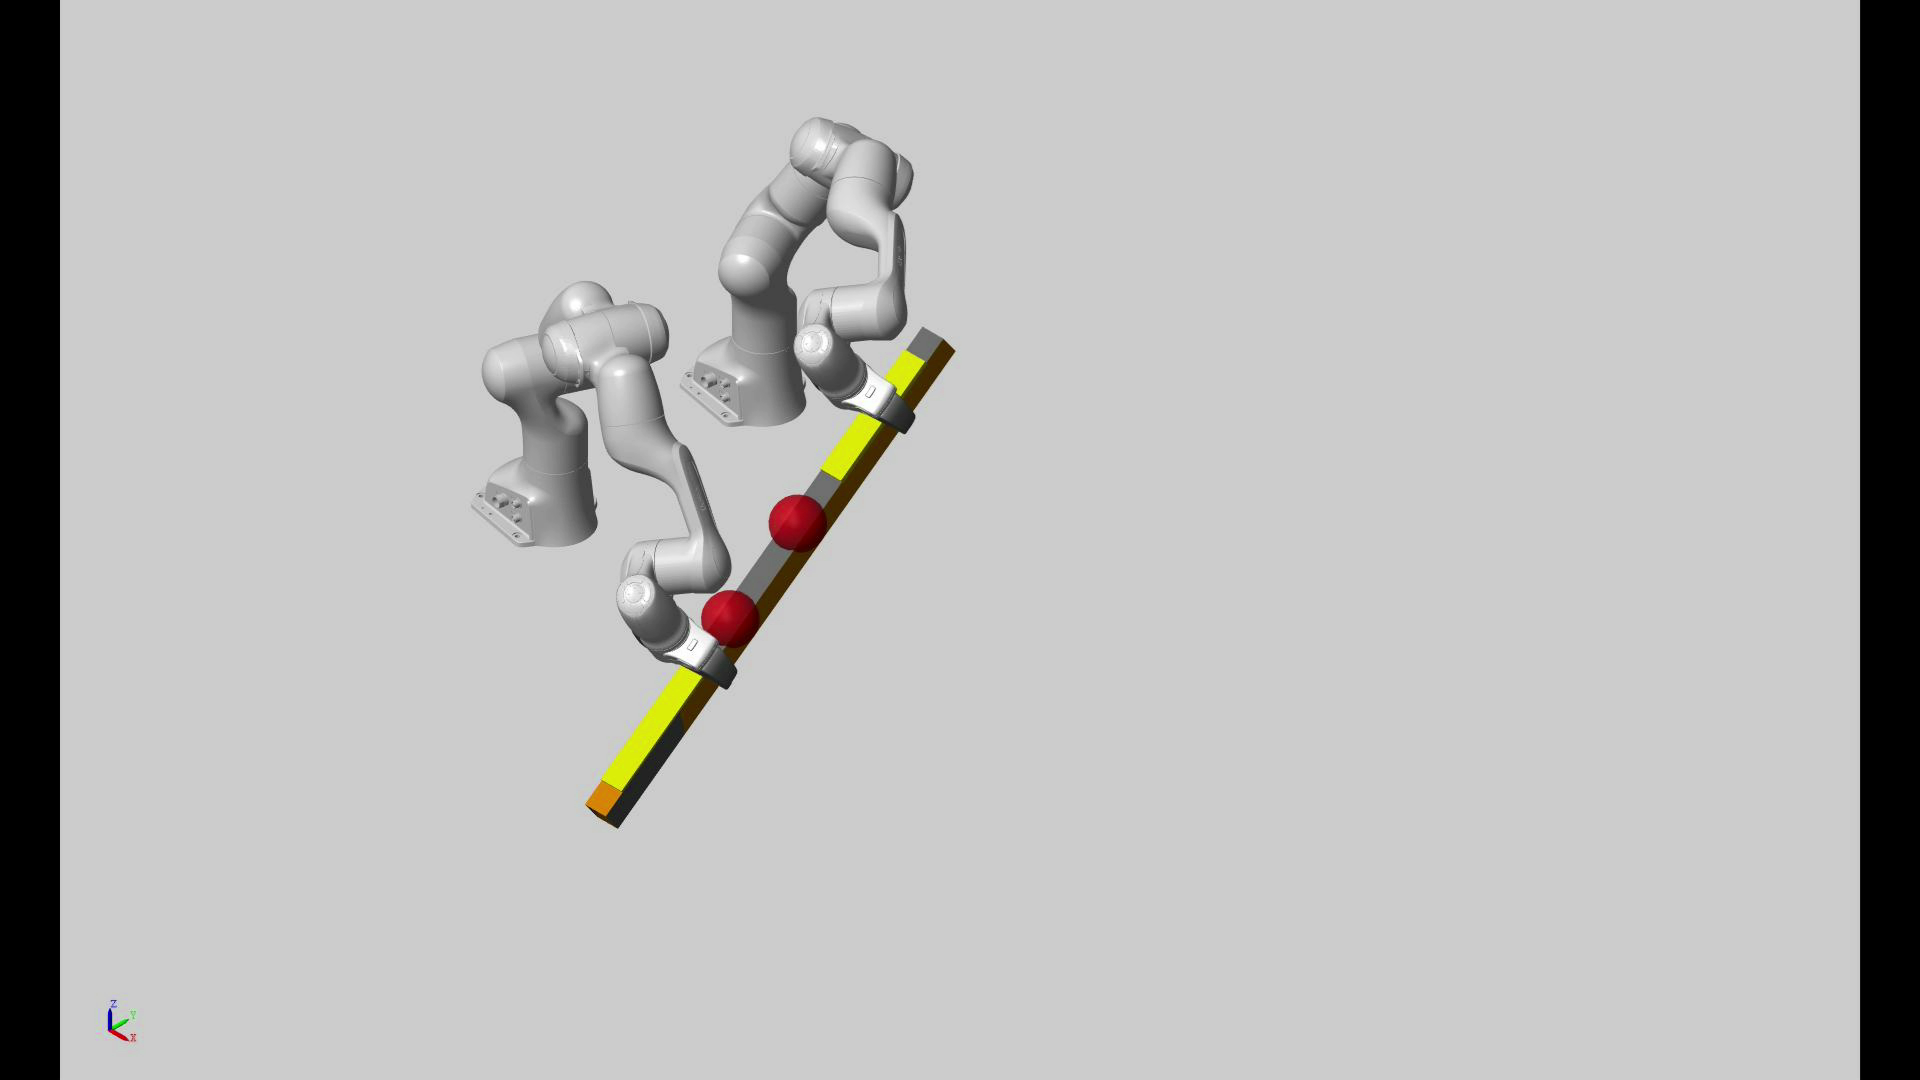
\includegraphics[width=0.32\columnwidth]{6}
	\caption{Simulation snapshots showing multi-robot handover with different perspectives. One compact QP formulation handles three robot: the object and two Panda robotic arms. Each Panda is tracking its corresponding grasping-set (highlighted in yellow) formulated as described in \cref{subsec-chap4:grasping-set-tracking}. The actual object is shown in gray and tracked by the observed object shown in orange as described in \cref{subsec-chap4:observation task}. The red spheres denote the placement of the human hands holding the object.}
	\label{fig:multi-robot handover}
\end{figure}

\section{Conclusion}\label{sec-chap4:conclusion}
In this chapter, we proposed an original approach for human-robot handovers formulation using task-space optimization controller. The main idea behind our approach is a novel implementation of the tasks interdependency, which consists in providing the output of a task (of an estimation nature) as an input to another task so that both meet at the handover spot without explicit time or handover position specification. Our experimental results confirmed very promising performances of simple handovers focusing mainly on the reaching phase.

This new approach raised very promising novel features of the task-space optimization control schemes. Extension in terms of functionalities and theoretical investigation on how observer-tasks can be embedded through task interdependencies and constraints between task errors might open perspectives in embedding scheduling in the task-space formalism. Our ongoing and future research focuses on this issue with complete phases and more complex handovers considering force cues. 



%QP is one of the most used tools used to solve the multi-objective control problem (either by following a soft or strict hierarchy) by finding the optimal decision variables  $\decisionVector$ that minimize, at the best, all the tasks errors. Classically, each task converges toward its own reference which is either operator-defined or provided by a planner. In addition, the tasks are generally meant to achieve control objectives that are independent of each other. 

%In this chapter, we introduce the idea of \emph{interdependent tasks}: the output of one task is the reference of another task. To exemplify this new concept, we propose to apply for bi-directional human-robot handover formulation using task-space QP. 